\chapter{Analysis}
\label{Analyse}

Since HDC includes randomness by design, the final classification results fluctuate slightly with the initial state of the \ac{RNG}, which is used to initialize the CCIM through random vectors and feature-specific random permutations. Therefore, all algorithmic accuracy experiments in Sections \ref{sec:results_baseline} to \ref{sec:combined_results} are conducted five times with the seeds 1, 2, 3, 4, and 5, and the reported accuracies are averaged over these five runs. Although a higher number of seeds would improve statistical robustness, five runs are used as a trade-off because of the long runtimes, especially for large vector dimensions and GA optimization, where thousands of HDC models have to be generated, trained, and evaluated per seed.

All experiments use the four datasets described in Section \ref{sec:emg-preprocessing}. The 870 test samples are kept fixed. From the remaining data, 30\% of the samples of each class are separated for validation, resulting in 3,040 training and 1,300 validation samples. The validation set is used only for GA optimization. However, the same train-validation split is also kept for experiments without GA to ensure that all experiments use the same amount of training data.

The accuracy is first determined separately for each of the four datasets. The dataset-average accuracy is then calculated as the arithmetic mean of the four individual dataset accuracies. Results for the individual datasets are additionally provided where relevant differences are observed. N-grams containing transitions between different movement classes are excluded from the primary accuracy results.


\section{Baseline HDC Model Results}
\label{sec:results_baseline}

This section evaluates the baseline HDC model to establish the reference configuration for the following optimization experiments.
But before that, the previously chosen size of N-grams $N$ needs to be justified. Figure~\ref{fig:ngram} shows the influence of the N-gram size on the baseline HDC model with $D=10,000$ and $L=40$. Compared to classification without temporal context at $N=1$, where only the current spatially encoded sample is used, the mean accuracy increases from $94.14\%$ to $94.78\%$ for $N=3$. For larger N-gram sizes, however, the accuracy does not increase substantially. The highest measured value is obtained for $N=9$ with $94.89\%$, which is only $0.1145$ percentage points above the result for $N=3$. Therefore, $N=3$ is selected as the baseline N-gram size. This choice does not maximize the measured accuracy over all tested values, but it provides almost the same classification performance while using a much shorter temporal context, and therefore a smaller N-gram buffer and less temporal encoding overhead. This trade-off is preferred over the marginal accuracy gain achieved with larger N-gram sizes, because the following experiments focus on reducing the computational cost of the HDC model.

\begin{figure}[htbp]
    \centering
    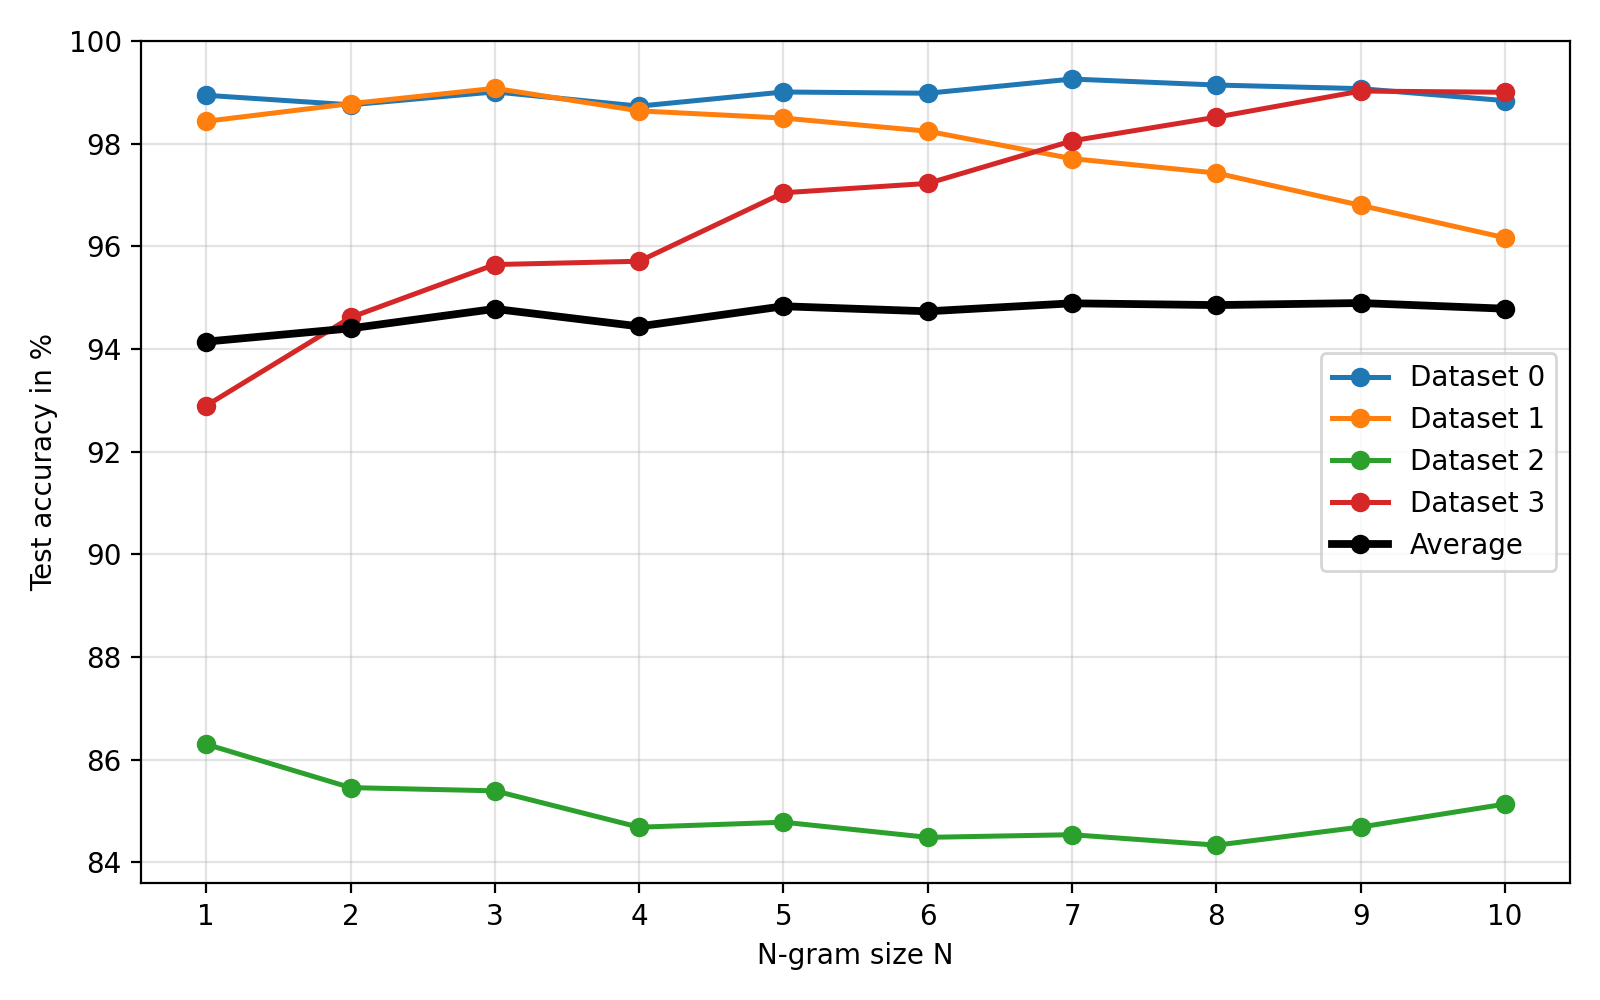
\includegraphics[width=\textwidth]
    {Images/ngram.png}
    \caption{Mean classification accuracy of the baseline HDC model for different N-gram sizes. The vector dimension is fixed to $D=10{,}000$, the number of CCIM levels to $L=40$, and uniform quantization is used. The reported accuracies are averaged over the four datasets and five seeds.}
    \label{fig:ngram}
\end{figure}
%python3 analysis/ngram_size_sweep/plot_ngram_accuracy.py --min-ngram 1 --max-ngram 10






 
Table~\ref{tab:baseline_accuracy} shows the accuracy of the baseline HDC model with $D=10{,}000$ and $L=40$. Between datasets, clear differences are apparent. Datasets~0 and~1 achieve the highest accuracies, depending on the seed, while Dataset~2 consistently performs worst. Ledwig \cite{ledwig_vdl-implementierung_2025} analyzed the datasets with PCA and concluded that these differences emerge from the data itself, because in Dataset 2, samples from different classes show a strong overlap and are thus not clearly distinguishable. 

Some variation is also visible across the different seeds. As described above, this results from the different \ac{RNG} initializations used to generate the \ac{CCIM}. The last column of Table \ref{tab:baseline_accuracy} shows the mean and standard deviation across all seeds. This mean across seeds is used in the following experiments as the main metric for the dataset. The maximum difference between seeds is below 1.1 percentage points for all datasets, and the standard deviation ranges from 0.22 to 0.43 percentage points. On average across all datasets, the model achieves 94.781\% accuracy with $L=40$ and $D=10{,}000$ dimensions, which will serve as a reference point for later evaluation.



\begin{table}[htbp]
    \centering
    \caption{Classification accuracy of the baseline HDC model for each dataset and seed. The final column reports the mean and sample standard deviation across the five runs.}
    \label{tab:baseline_accuracy}
    \begin{tabular}{c c c c c c c}
        \toprule
        \textbf{Dataset}
        & \textbf{Seed 1}
        & \textbf{Seed 2}
        & \textbf{Seed 3}
        & \textbf{Seed 4}
        & \textbf{Seed 5}
        & \textbf{Mean $\pm$ SD} \\
        \midrule
        0 & 98.96\% & 98.96\% & 99.19\% & 99.31\% & 98.62\% & 99.01\% $\pm$ 0.27\% \\
        1 & 99.08\% & 99.08\% & 99.42\% & 98.85\% & 98.96\% & 99.08\% $\pm$ 0.22\% \\
        2 & 85.37\% & 85.02\% & 85.83\% & 85.14\% & 85.60\% & 85.39\% $\pm$ 0.33\% \\
        3 & 95.51\% & 95.97\% & 95.16\% & 96.20\% & 95.39\% & 95.65\% $\pm$ 0.43\% \\
        \bottomrule
    \end{tabular}
\end{table}
Figure~\ref{fig:baseline_dimension_sweep} shows the classification accuracy of the baseline model for vector dimensions from $D=201$ to $D=20{,}000$ at a fixed number of $L=40$ \ac{CCIM} levels. Since no measured accuracy falls below $70\%$, the y-axis is limited to the range from $70\%$ to $100\%$. The vector dimension is evaluated in steps of 100 below $D=1{,}000$, 500 between $D=1{,}000$ and $D=10{,}000$, and 1,000 from $D=10{,}000$ to $D=20{,}000$.
\begin{figure}[htbp]
    \centering
    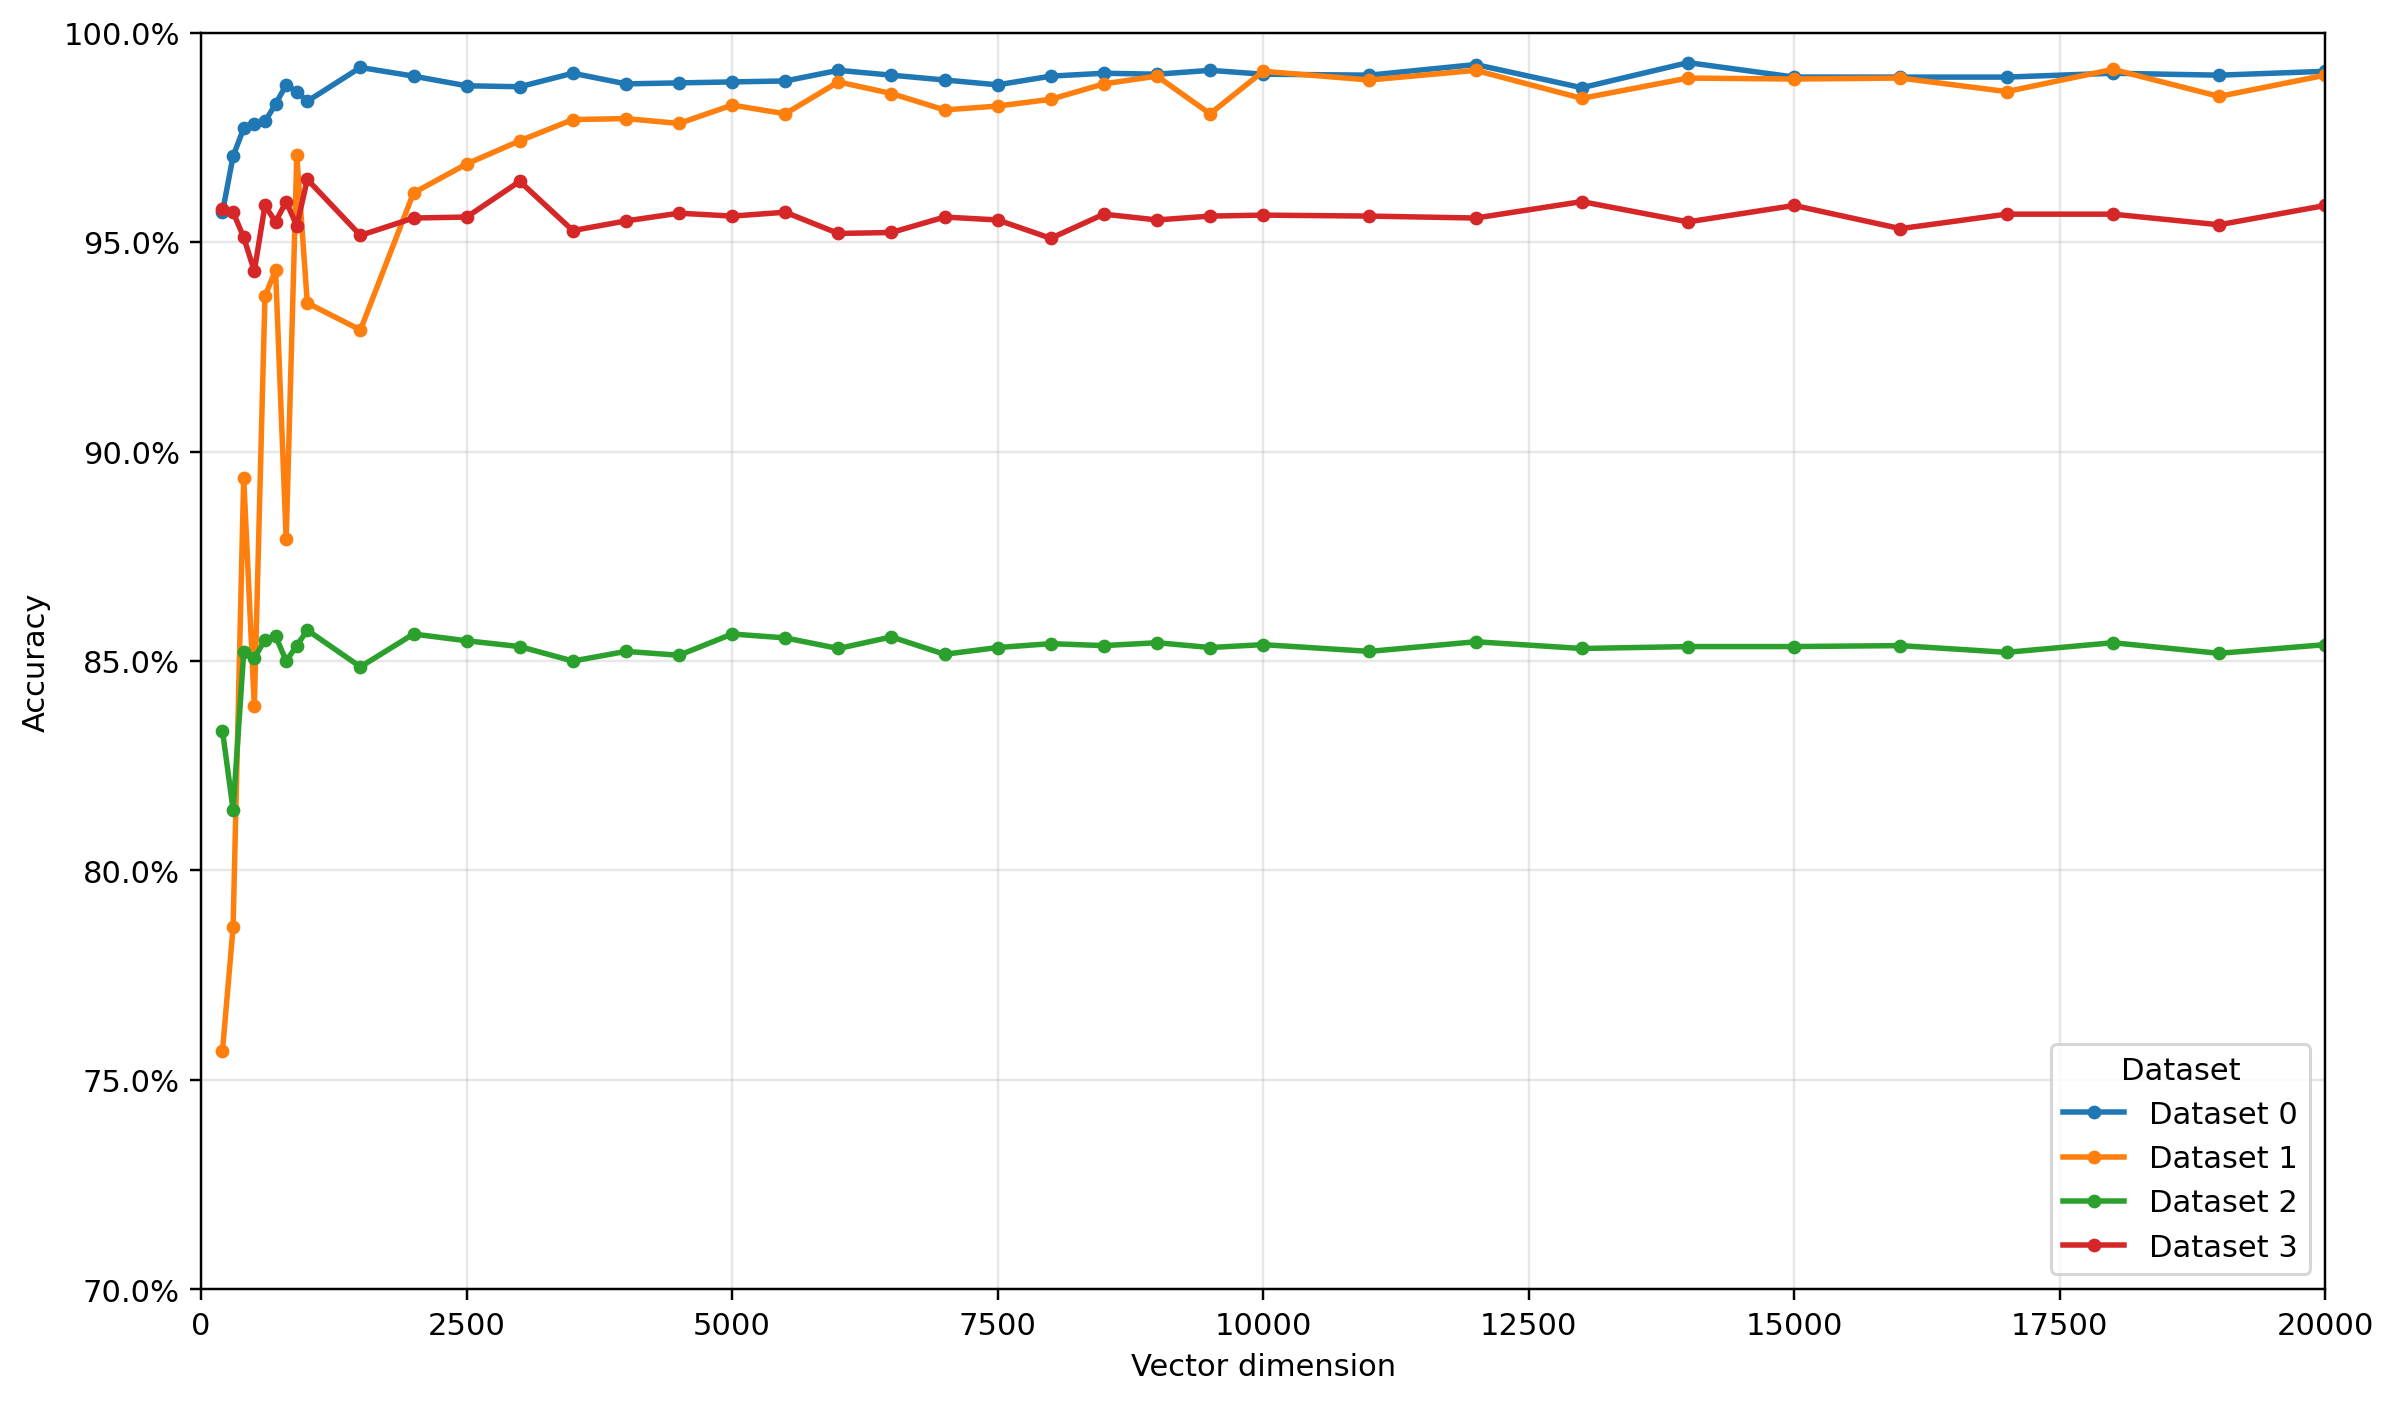
\includegraphics[width=\textwidth]
    {Images/baseline_lvl40_full.png}
    \caption{Classification accuracy of the baseline HDC model at vector dimensions from $D=201$ to $D=20{,}000$ with $L=40$ for each dataset.}
    \label{fig:baseline_dimension_sweep}
\end{figure}%python3 analysis/benchmarking/baseline/scripts/plot_accuracy_by_dimension.py --num-levels 40 --min-dimension 0 --max-dimension 20000 --output Images/baseline_lvl40_full.png
Despite the large differences in absolute accuracy across datasets, a clear trend is visible within each dataset. While low dimensions generally result in lower accuracy, the accuracy initially increases with $D$ and then saturates, such that further increases in the vector dimension provide little additional improvement. This saturation behavior also supports the choice of $D=10{,}000$ as the baseline vector dimension in this work. Comparing $D=10{,}000$ with $D=20{,}000$ shows an average accuracy increase of only 0.052 percentage points across all four datasets. The largest increase is observed for Dataset~0 with $+0.069$ percentage points, while Dataset~1 even shows a slight decrease of $0.092$ percentage points. Therefore, increasing the dimension beyond $D=10{,}000$ increases the dimension-dependent computational effort while providing only a negligible accuracy improvement on average.

On the other hand, halving the vector dimension to $D=5{,}000$ approximately halves the hypervector storage and the computational effort of operations that scale linearly with $D$. However, the average accuracy is only $0.19$ percentage points lower, with the largest decrease of $0.81$ percentage points for Dataset~1, while Dataset~2 even shows a slight increase of $0.25$ percentage points. This suggests that reducing the vector dimension by a factor of two can substantially reduce vector-dependent memory and computation while causing only a small loss in average classification accuracy. Whether \ac{CCIM} optimization and quantization can compensate for this accuracy loss at lower vector dimensions is investigated in Chapters~\ref{sec:GA_results} to~\ref{sec:combined_results}.

Figure~\ref{fig:baseline_dimension_low} shows the same experiment as Figure~\ref{fig:baseline_dimension_sweep}, but at a higher resolution of 20 dimensions and a focus on low vector dimensions from $D=201$ to $D=5{,}000$. At low vector dimensions, even small changes in $D$ can result in significant fluctuations in classification accuracy. As the vector dimension approaches $D=5{,}000$, these fluctuations become smaller. This behavior is consistent with the increased redundancy of higher-dimensional representations, in which individual dimensions have less influence on the overall representation.

The accuracy degradation at very low vector dimensions is again strongly dataset-dependent. As shown in Figure~\ref{fig:baseline_dimension_low}, the accuracies of Datasets~0, 2, and 3 at $D=1{,}000$ remain close to those at $D=5{,}000$. Datasets~2 and 3 even perform slightly better at $D=1{,}000$, while Dataset~0 performs slightly worse, but all three differences remain below one percentage point. Dataset~1, in contrast, shows a decrease of $4.72$ percentage points when reducing the vector dimension from $D=5{,}000$ to $D=1{,}000$. Below $D=1{,}000$, only Dataset~3 mostly preserves its accuracy, with a decrease of only $0.71$ percentage points at $D=201$. The other datasets show larger accuracy losses, with Dataset~1 being affected most strongly. Consequently, the dataset-average accuracies at $D=201$ and $D=1{,}000$ are $87.63\%$ and $93.54\%$, respectively, corresponding to decreases of $7.15$ and $1.24$ percentage points relative to the $D=10{,}000$ baseline.

\begin{figure}[htbp]
    \centering
    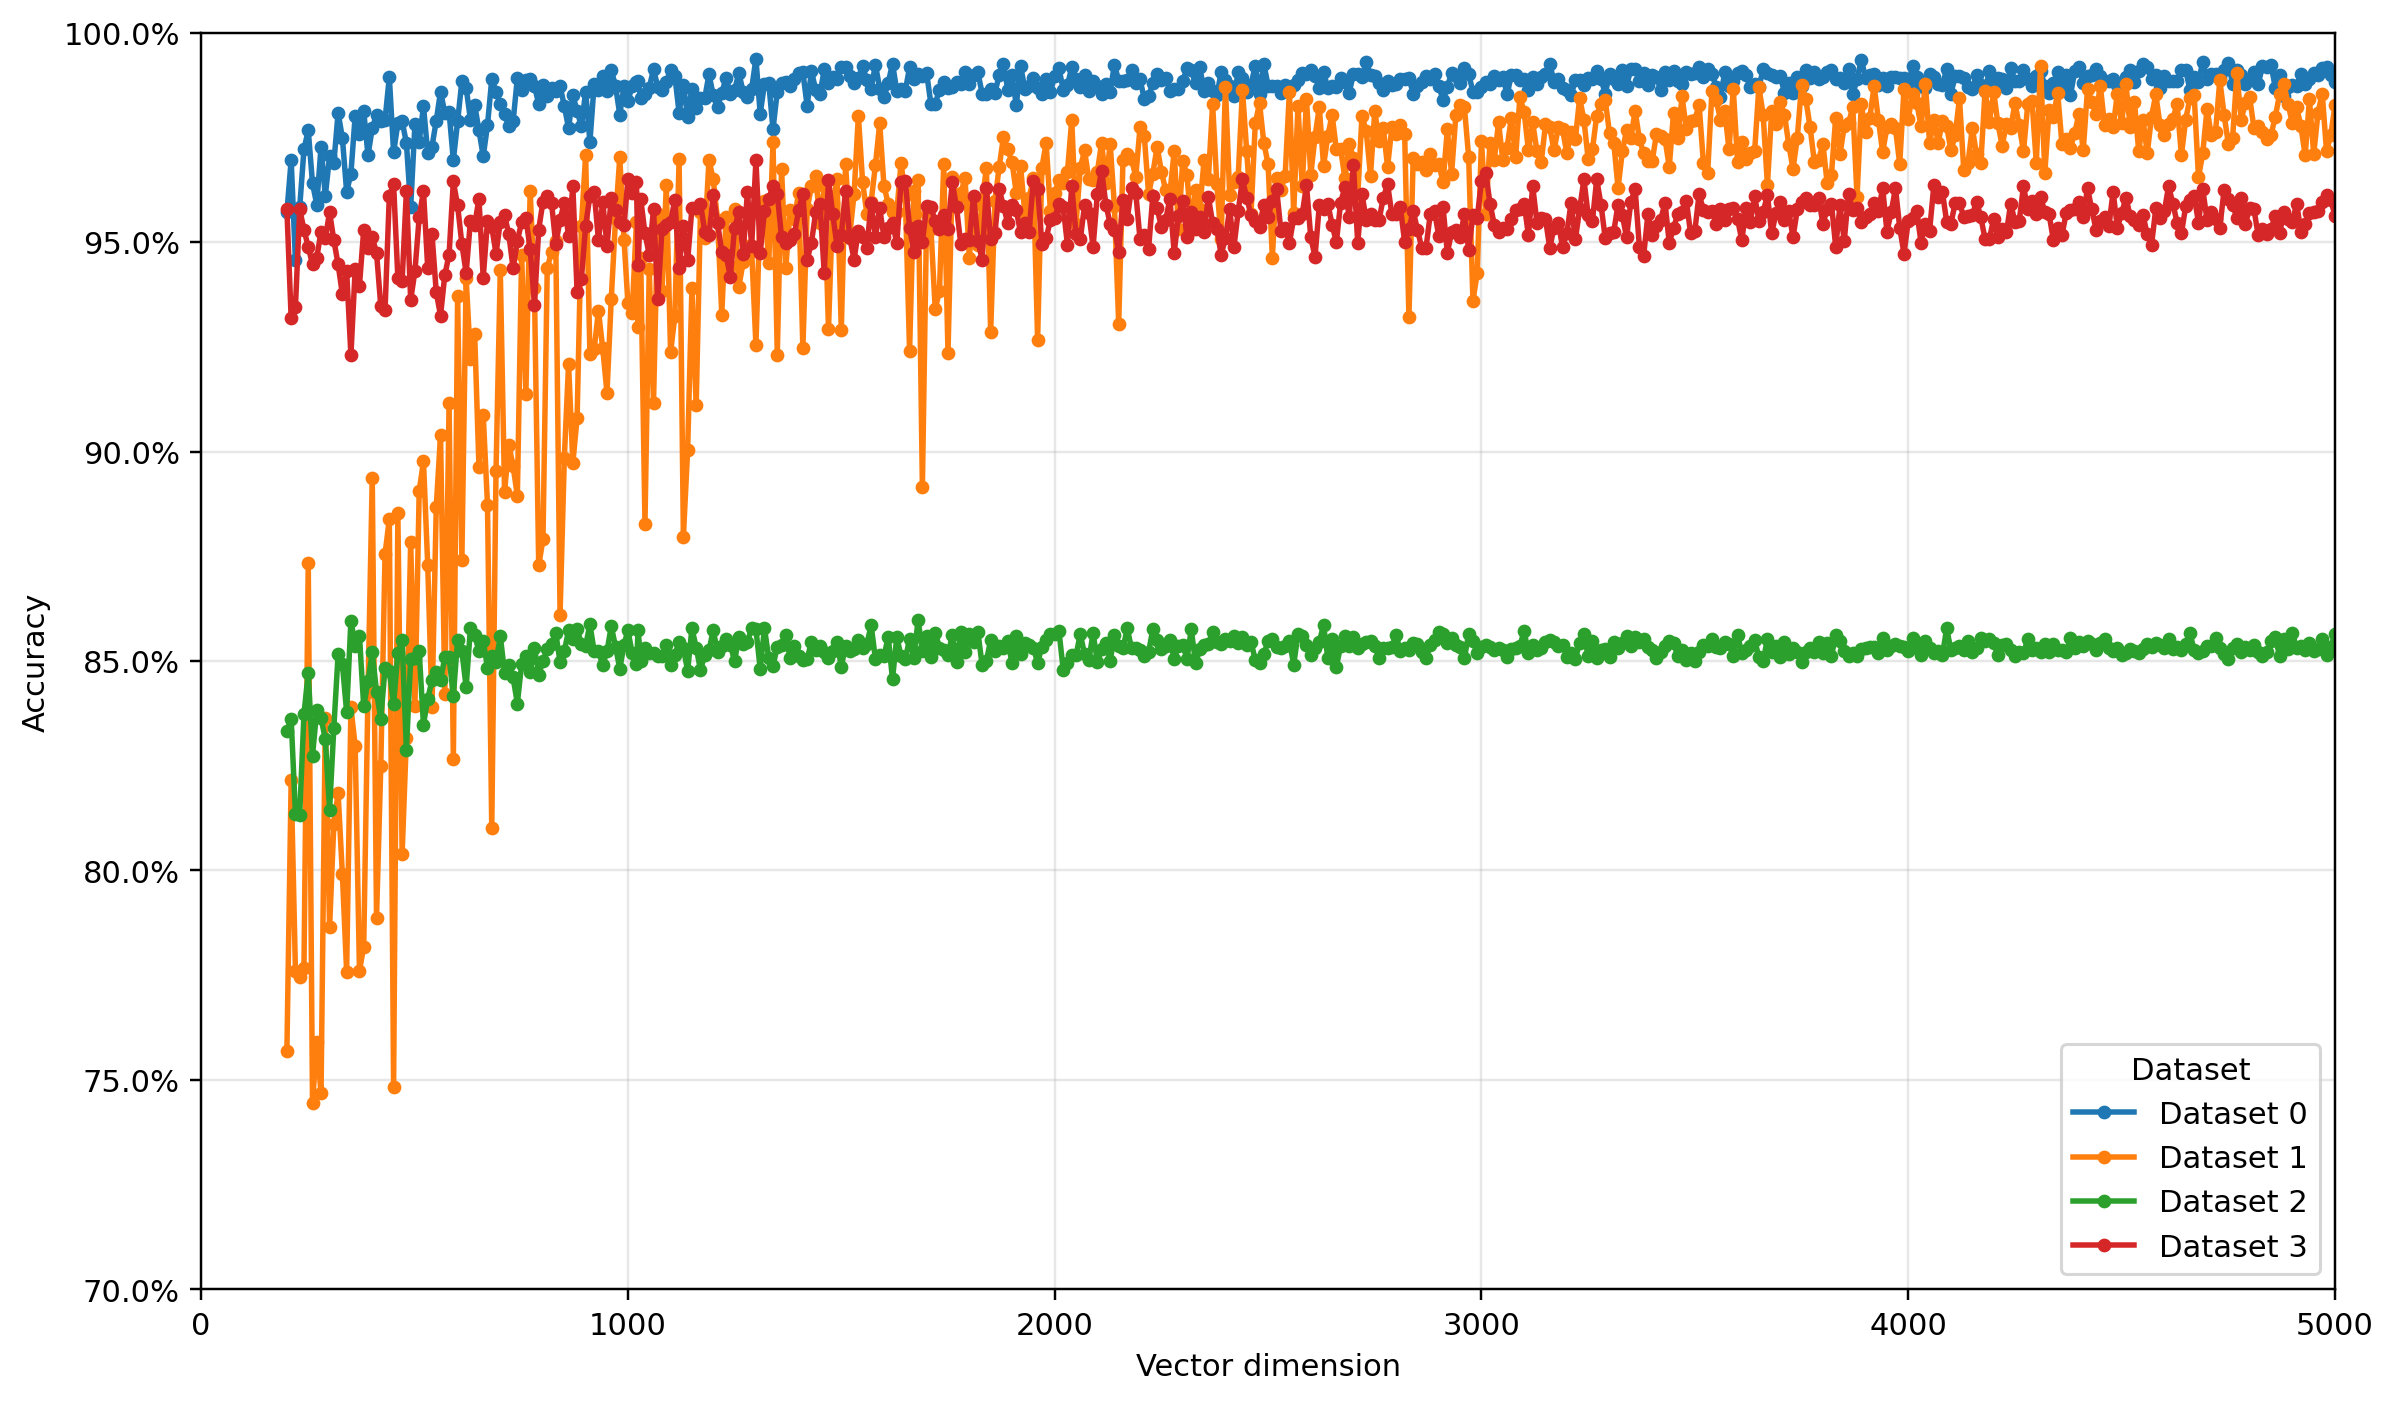
\includegraphics[width=\textwidth]
    {Images/baseline_lvl40_lowDims.png}
    \caption{Classification accuracy of the baseline HDC model at low vector dimensions with $L=40$ for each dataset.}
    \label{fig:baseline_dimension_low}
\end{figure}%python3 analysis/benchmarking/baseline/scripts/plot_accuracy_by_dimension.py --num-levels 40 --min-dimension 0 --max-dimension 5000 --dimension-grid all --output Images/baseline_lvl40_lowDims.png

%numlevels sweep
Figure~\ref{fig:baseline_levels} shows the classification accuracy as a function of the number of \ac{CCIM} levels from $L=5$ to $L=200$ at a fixed vector dimension of $D=10{,}000$. For small numbers of levels, the accuracy decreases for all datasets, as the coarse quantization provides insufficient resolution to represent relevant variations in the feature values. For Datasets~0 and 2, this degradation is mainly observed below approximately $L=13$ and $L=12$, respectively, while for Dataset~3 it extends to approximately $L=26$. For Datasets~0, 2, and 3, the accuracy eventually reaches a region in which further increases in $L$ provide little or no systematic improvement. The specific number of quantization levels $L$ of this point differs between datasets. For Datasets~0 and 2 it occurs at approximately $L=30$, while for Dataset~3 it occurs at approximately $L=64$. Between those regions, the accuracy varies nonlinearly with $L$. This suggests that the placement of the uniform quantization thresholds interacts with the feature distributions, such that some level counts may align better with discriminative regions of the data than others.
Dataset 1 is a strong outlier here. Its accuracy varies nonlinearly across the tested level counts, with local maxima around $L=40$, $L=100$, and $L=160$. This strong dependence on $L$ suggests that Dataset~1 is particularly sensitive to the alignment of the quantization thresholds and is therefore an important target for quantization optimization. In contrast to the other datasets, no comparable high-accuracy saturation region is observed. An extended experiment up to $L=500$ (not shown) further showed that the accuracy obtained at $L=40$ was not reached again at larger level counts.

\begin{figure}[htbp]
    \centering
    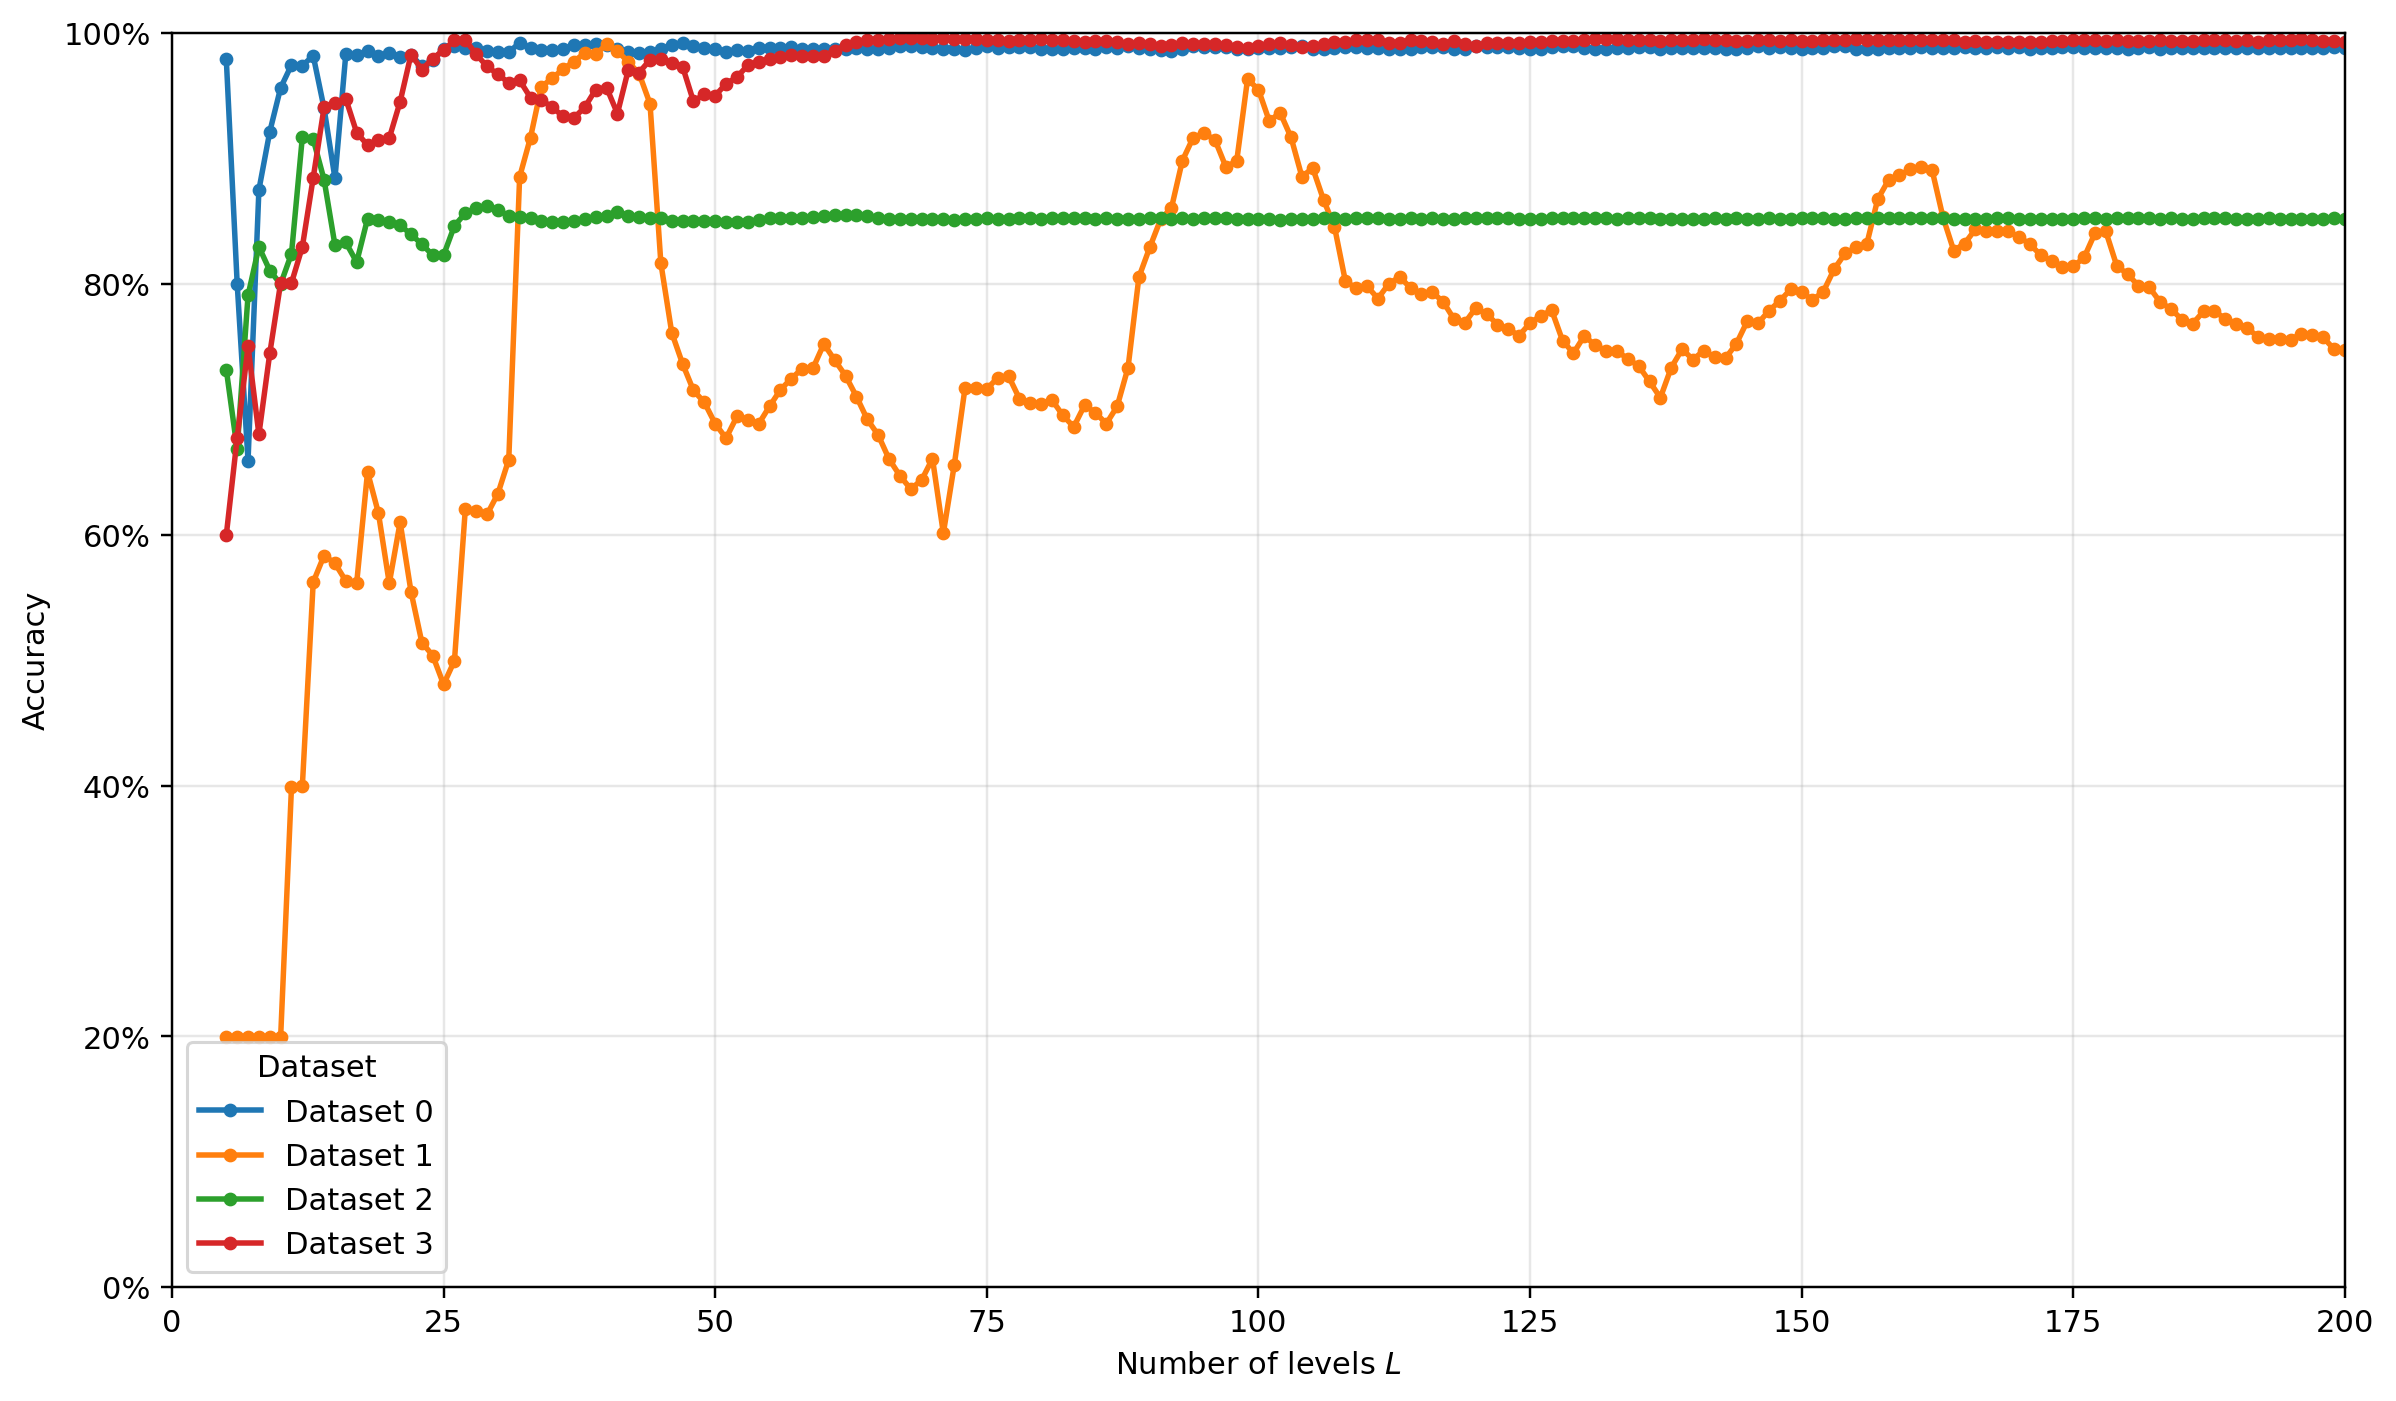
\includegraphics[width=\textwidth]
    {Images/baseline_dim10k_full.png}
    \caption{Classification accuracy of the baseline HDC model for different numbers of \ac{CCIM} levels at $D=10{,}000$.}
    \label{fig:baseline_levels}
\end{figure}

The results also show that the dependence of classification accuracy on both $D$ and $L$ is dataset-specific and nonlinear. Although increasing either parameter generally improves accuracy at low values, local maxima and saturation regions occur at different parameter values for the individual datasets. Consequently, no single tested value of $D$ or $L$ provides the best accuracy for all datasets.


\section{Results of Genetic Optimization}
\label{sec:GA_results}

The previous section showed that reducing the vector dimension can strongly reduce the model cost, but also that the baseline model loses accuracy at low dimensions. This section evaluates whether the GA-based CCIM optimization can compensate for this loss. The number of quantization levels is kept fixed at $L=40$, and uniform quantization is used, so that the distribution of the level hypervectors in the CCIM is the only changed property.

Before comparing the optimized model on the test set, the optimization process itself is analyzed. Figure~\ref{fig:ga_convergence} shows a representative convergence analysis on the example of Dataset~3 with $D=10{,}000$ averaged across five seeds. The upper plot shows the best and mean validation accuracy of the population per generation, while the lower plot shows how many newly generated individuals are selected into the next generation.

\begin{figure}[htbp]
    \centering
    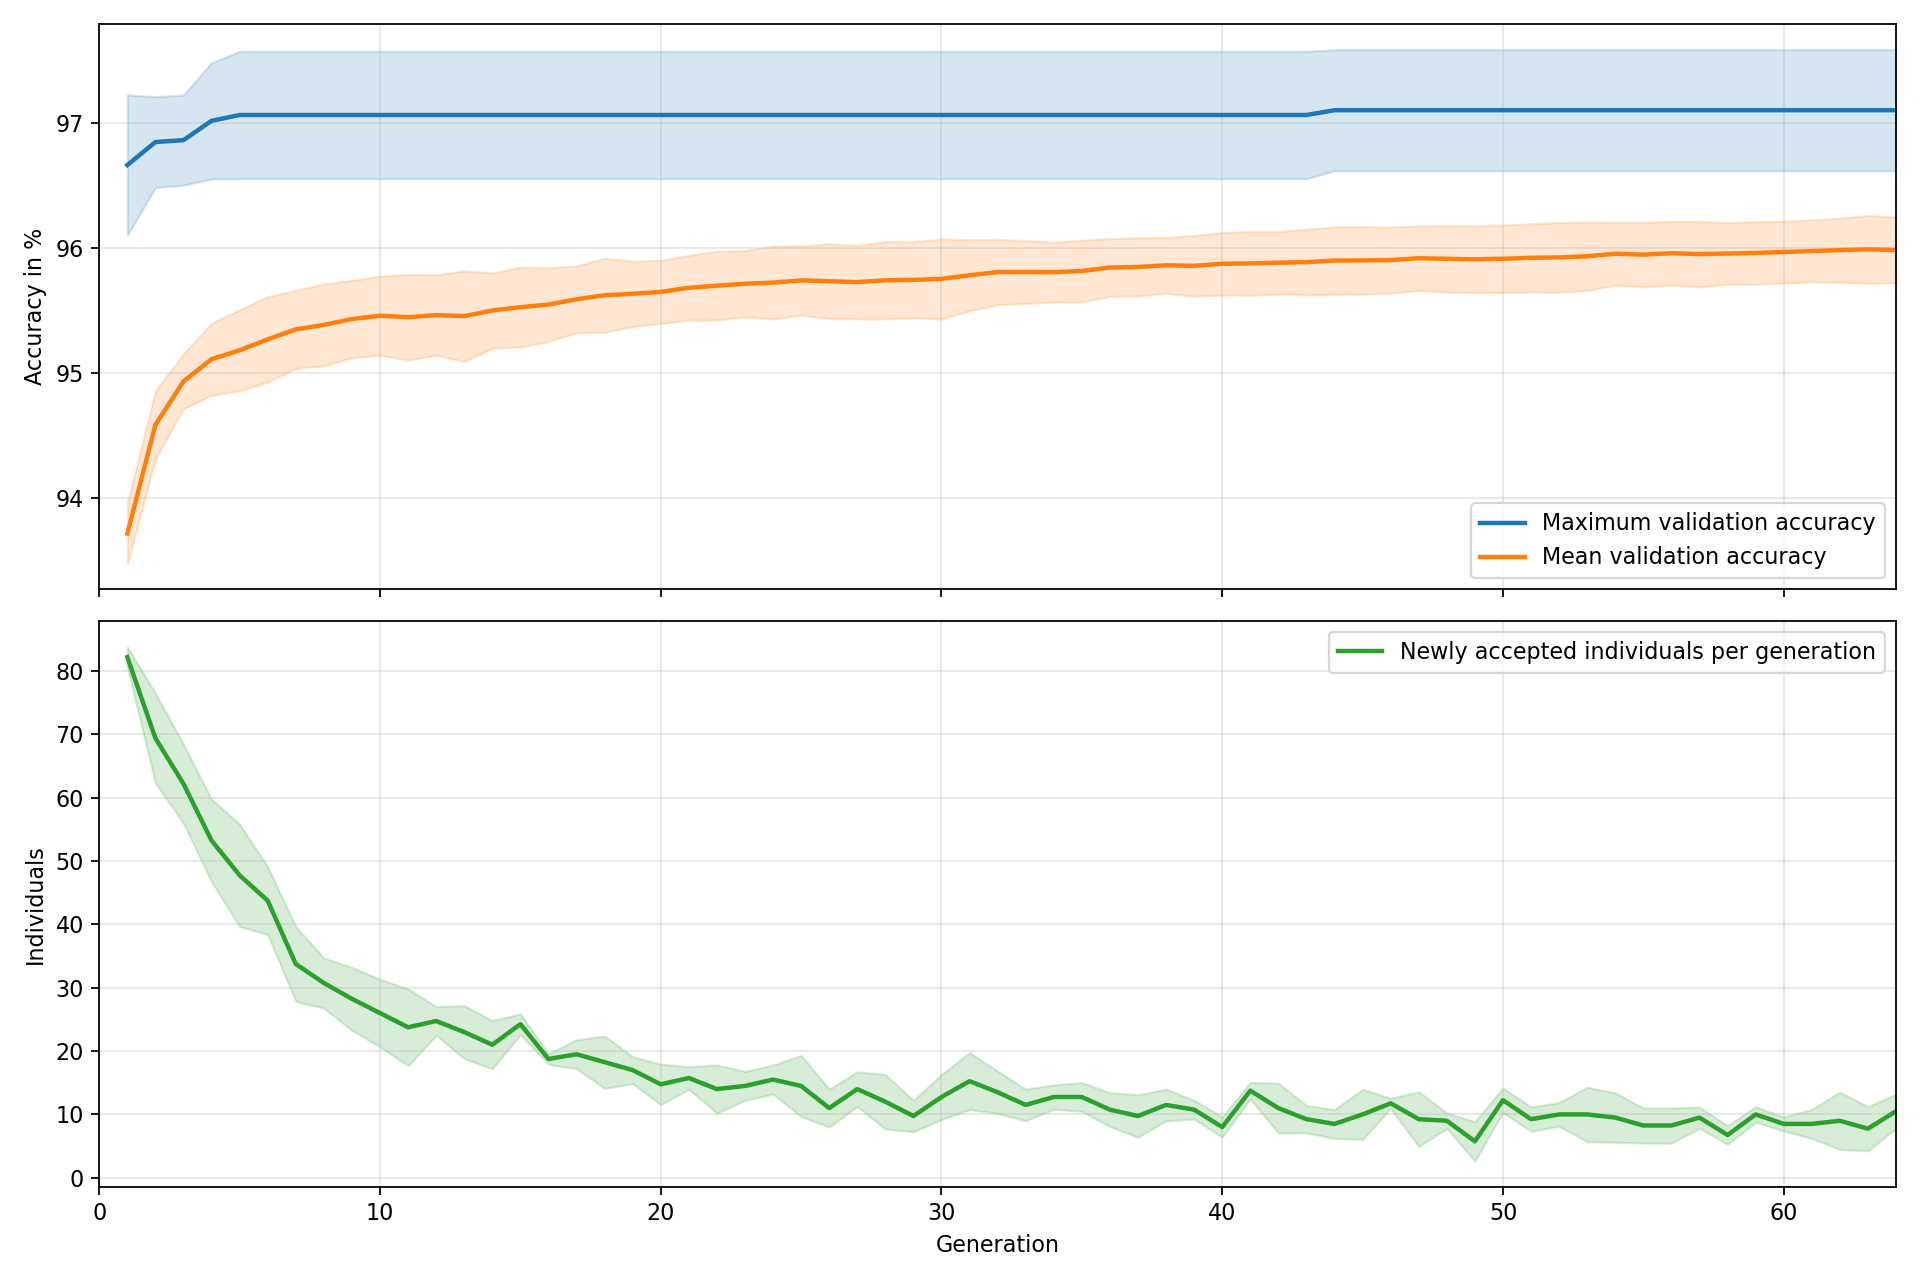
\includegraphics[width=\textwidth]
    {Images/ga_convergence.png}
    \caption{Convergence behavior of the GA-based CCIM optimization for Dataset~3 with $D=10{,}000$ and $L=40$. The upper plot shows the maximum and mean validation accuracy of the population, while the lower plot shows the number of newly accepted individuals per generation.}
    \label{fig:ga_convergence}
\end{figure}%python3 analysis/CiM_evaluation/plot_ga_run_convergence.py   --logs analysis/CiM_evaluation/dataset3_ga_cim_exports/output_dataset03_seed*_l40_d10000.txt   --show
%Dataset 3, 5 seeds, 64 gen 128 pop

The convergence behavior shows that the GA performs most of its exploration in the early generations. During this phase, many offspring are selected into the next generation, which indicates that the population still has significant room for improvement and that newly generated CCIM configurations frequently outperform existing ones. This is also reflected in the rapid increase of the best validation accuracy during the first generations.

In later generations, the optimization shifts from broad exploration to refinement. The best validation accuracy changes only minimally after the early improvement phase, while the mean population accuracy continues to increase. This indicates that the population becomes more concentrated around high-performing CCIM configurations. At the same time, the number of newly accepted individuals decreases strongly, showing that fewer offspring are selected into the next generation. Overall, the GA therefore shows as expected a clear convergence trend, while a small number of newly generated individuals is still selected in later generations.\\


To analyze how the GA actually changes the structure of the CCIM, an optimized bit-flip distribution is visualized in Figure~\ref{fig:CCIM_optimized}. It results from the final selected bit-flip matrix $\mathbf{B}^{\ast}$ for Dataset~3 and seed 1 included in the convergence analysis of Figure \ref{fig:ga_convergence}. For each transition $i$ between two neighboring level hypervectors, the plot reports how many bits are flipped. The blue lines show the feature-specific bit-flip counts, the red line shows the mean across all features, and the shaded region indicates the standard deviation across features. The dashed black line marks the equally spaced baseline.

\begin{figure}[htbp]
    \centering
    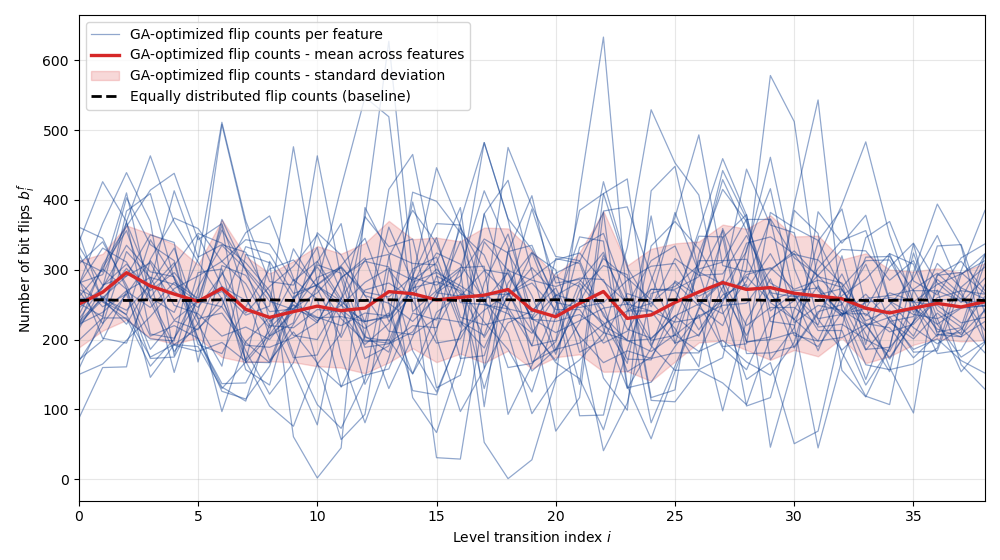
\includegraphics[width=\textwidth]
    {Images/CCIM_optimized.png}
    \caption{Optimized bit-flip distribution after GA optimization for Dataset~3. The blue lines show the feature-specific flip-count distributions, the red line shows the mean across features, and the shaded region shows the standard deviation across features. The dashed black line marks the equally spaced baseline.}
    \label{fig:CCIM_optimized}
\end{figure}
%RUN="$(basename "$(ls -td CiMs/ga_run_*dataset03_seed01_l40_d10000_pop128_gen64 | head -1)")"

%python3 analysis/CiM_evaluation/analyze_ga_cim.py \
%  --run "$RUN" \
%  --generation 64 \
%  --individual 85 \
%  --reference-cim CiMs/naive_l40_d10000_seed01/generation_0000/cim_0000.csv \
%  --show

The equally spaced baseline distributes the flip budget almost uniformly over the $L-1=39$ transitions. Since $D/(L-1)=10{,}000/39 \approx 256.41$, the baseline uses 256 or 257 bit flips per transition. The optimized CCIM preserves the same total flip budget for every feature by construction. Consequently, the mean number of bit flips across the $L-1=39$ transitions of each feature remains approximately $256.41$.

This redistribution is highly feature-specific. Across all feature-transition pairs, the optimized bit-flip counts range from 1 to 633, with a standard deviation of 79.70. In contrast, the transition-wise mean across features remains much closer to the baseline, ranging only from 230.34 to 295.78 bit flips. This indicates that the GA does not reveal a global shift that affects all features in the same way. Instead, high and low bit-flip counts occur at different transitions for different features, so no simple global pattern, such as consistently larger distances at early or late transitions, is visible.

The optimized CCIM is, in summary, structurally different from the equally spaced baseline. Some neighboring levels are compressed to almost identical hypervectors, while other neighboring levels are separated by more than twice the baseline distance. Whether this modified CCIM geometry improves the final model performance is evaluated in the following analysis.\\

%Robustness:
Since the \ac{GA} jointly optimizes validation accuracy and class-vector similarity, the final population contains multiple non-dominated solutions representing different trade-offs between the two objectives. To analyze whether the robustness objective is meaningful beyond the validation set, the individuals on the first Pareto front of the final generation are additionally evaluated on the test set.

Table~\ref{tab:ga_pareto_front} summarizes this analysis for Dataset~3, seed 1, with $D=10{,}000$ and $L=40$. The Pareto front is constructed by maximizing the validation class-average accuracy and minimizing the class-vector similarity. Lower similarity corresponds to larger separation between the learned class vectors and is therefore used as a robustness-oriented objective.

\begin{table}[htbp]
    \centering
    \small
    \setlength{\tabcolsep}{4pt}
    \caption{First Pareto front of the final GA generation for Dataset~3, seed 1, with $D=10{,}000$ and $L=40$. For each individual, the table reports the class-vector similarity, validation accuracy, test accuracy, and the difference between test and validation accuracy.}
    \label{tab:ga_pareto_front}
    \begin{tabular}{c c c c c}
        \toprule
        \textbf{Individual} 
        & \textbf{Similarity} 
        & \textbf{Validation acc.} 
        & \textbf{Test acc.} 
        & \textbf{Test $-$ Val.} \\
        \midrule
        119 & 0.313 & 95.21\% & 97.00\% & +1.78 pp \\
        82  & 0.318 & 95.44\% & 97.24\% & +1.78 pp \\
        98  & 0.319 & 95.68\% & 97.35\% & +1.66 pp \\
        71  & 0.319 & 95.99\% & 97.47\% & +1.47 pp \\
        92  & 0.321 & 96.06\% & 97.35\% & +1.28 pp \\
        73  & 0.322 & 96.22\% & 97.93\% & +1.70 pp \\
        70  & 0.325 & 96.60\% & 98.04\% & +1.43 pp \\
        69  & 0.329 & 96.60\% & 98.16\% & +1.55 pp \\
        108 & 0.331 & 96.99\% & 98.16\% & +1.16 pp \\
        85  & 0.337 & 97.22\% & 98.27\% & +1.05 pp \\
        \bottomrule
    \end{tabular}
\end{table}

Within this Pareto front, the two objectives reveal a clear trade-off. Candidates with lower class-vector similarity show a larger improvement from validation to test accuracy. The Pearson correlation between similarity and the test-validation difference is $-0.803$, with a Spearman correlation of $-0.806$. This indicates that, among Pareto-optimal individuals, stronger class-vector separation is associated with a larger gain on unseen test data.

But at the same time, lower similarity does not directly lead to the highest absolute test accuracy. The correlation between similarity and absolute test accuracy is positive, with a Pearson correlation of $0.911$. This is caused by the structure of the Pareto front. Individuals with higher validation accuracy also tend to have higher test accuracy, even if their class-vector similarity is larger. Candidate~119 represents the robustness-oriented end of the front, with the lowest similarity and one of the largest test-over-validation gains, while Candidate~85 represents the accuracy-oriented end, with the highest validation and test accuracy.

Therefore, class-vector similarity provides a useful criterion within this Pareto front, as it exposes solutions with different trade-offs between validation accuracy and class-vector separation. However, it should not replace validation accuracy as the primary objective but rather be interpreted as a secondary criterion that helps expose alternative robust solutions within the final Pareto front.

Since this analysis is performed on one representative final Pareto front, the observed correlations should be interpreted as evidence for the usefulness of the similarity objective in this experiment rather than as a general proof of robustness for all datasets and configurations.

After analyzing the optimization process and the resulting CCIM structure, the final effect of the GA optimization is evaluated on the test set. Figure~\ref{fig:ga_only_comparison} compares the classification accuracy of the HDC model with a GA-optimized CCIM against the unoptimized equally spaced CCIM for different vector dimensions at $L=40$. The red curves show the test accuracy after GA optimization, while the blue curves show the corresponding unoptimized baseline. The dotted horizontal line marks the reference accuracy of the unoptimized model with $D=10{,}000$ and $L=40$.

\begin{figure}[htbp]
    \centering
    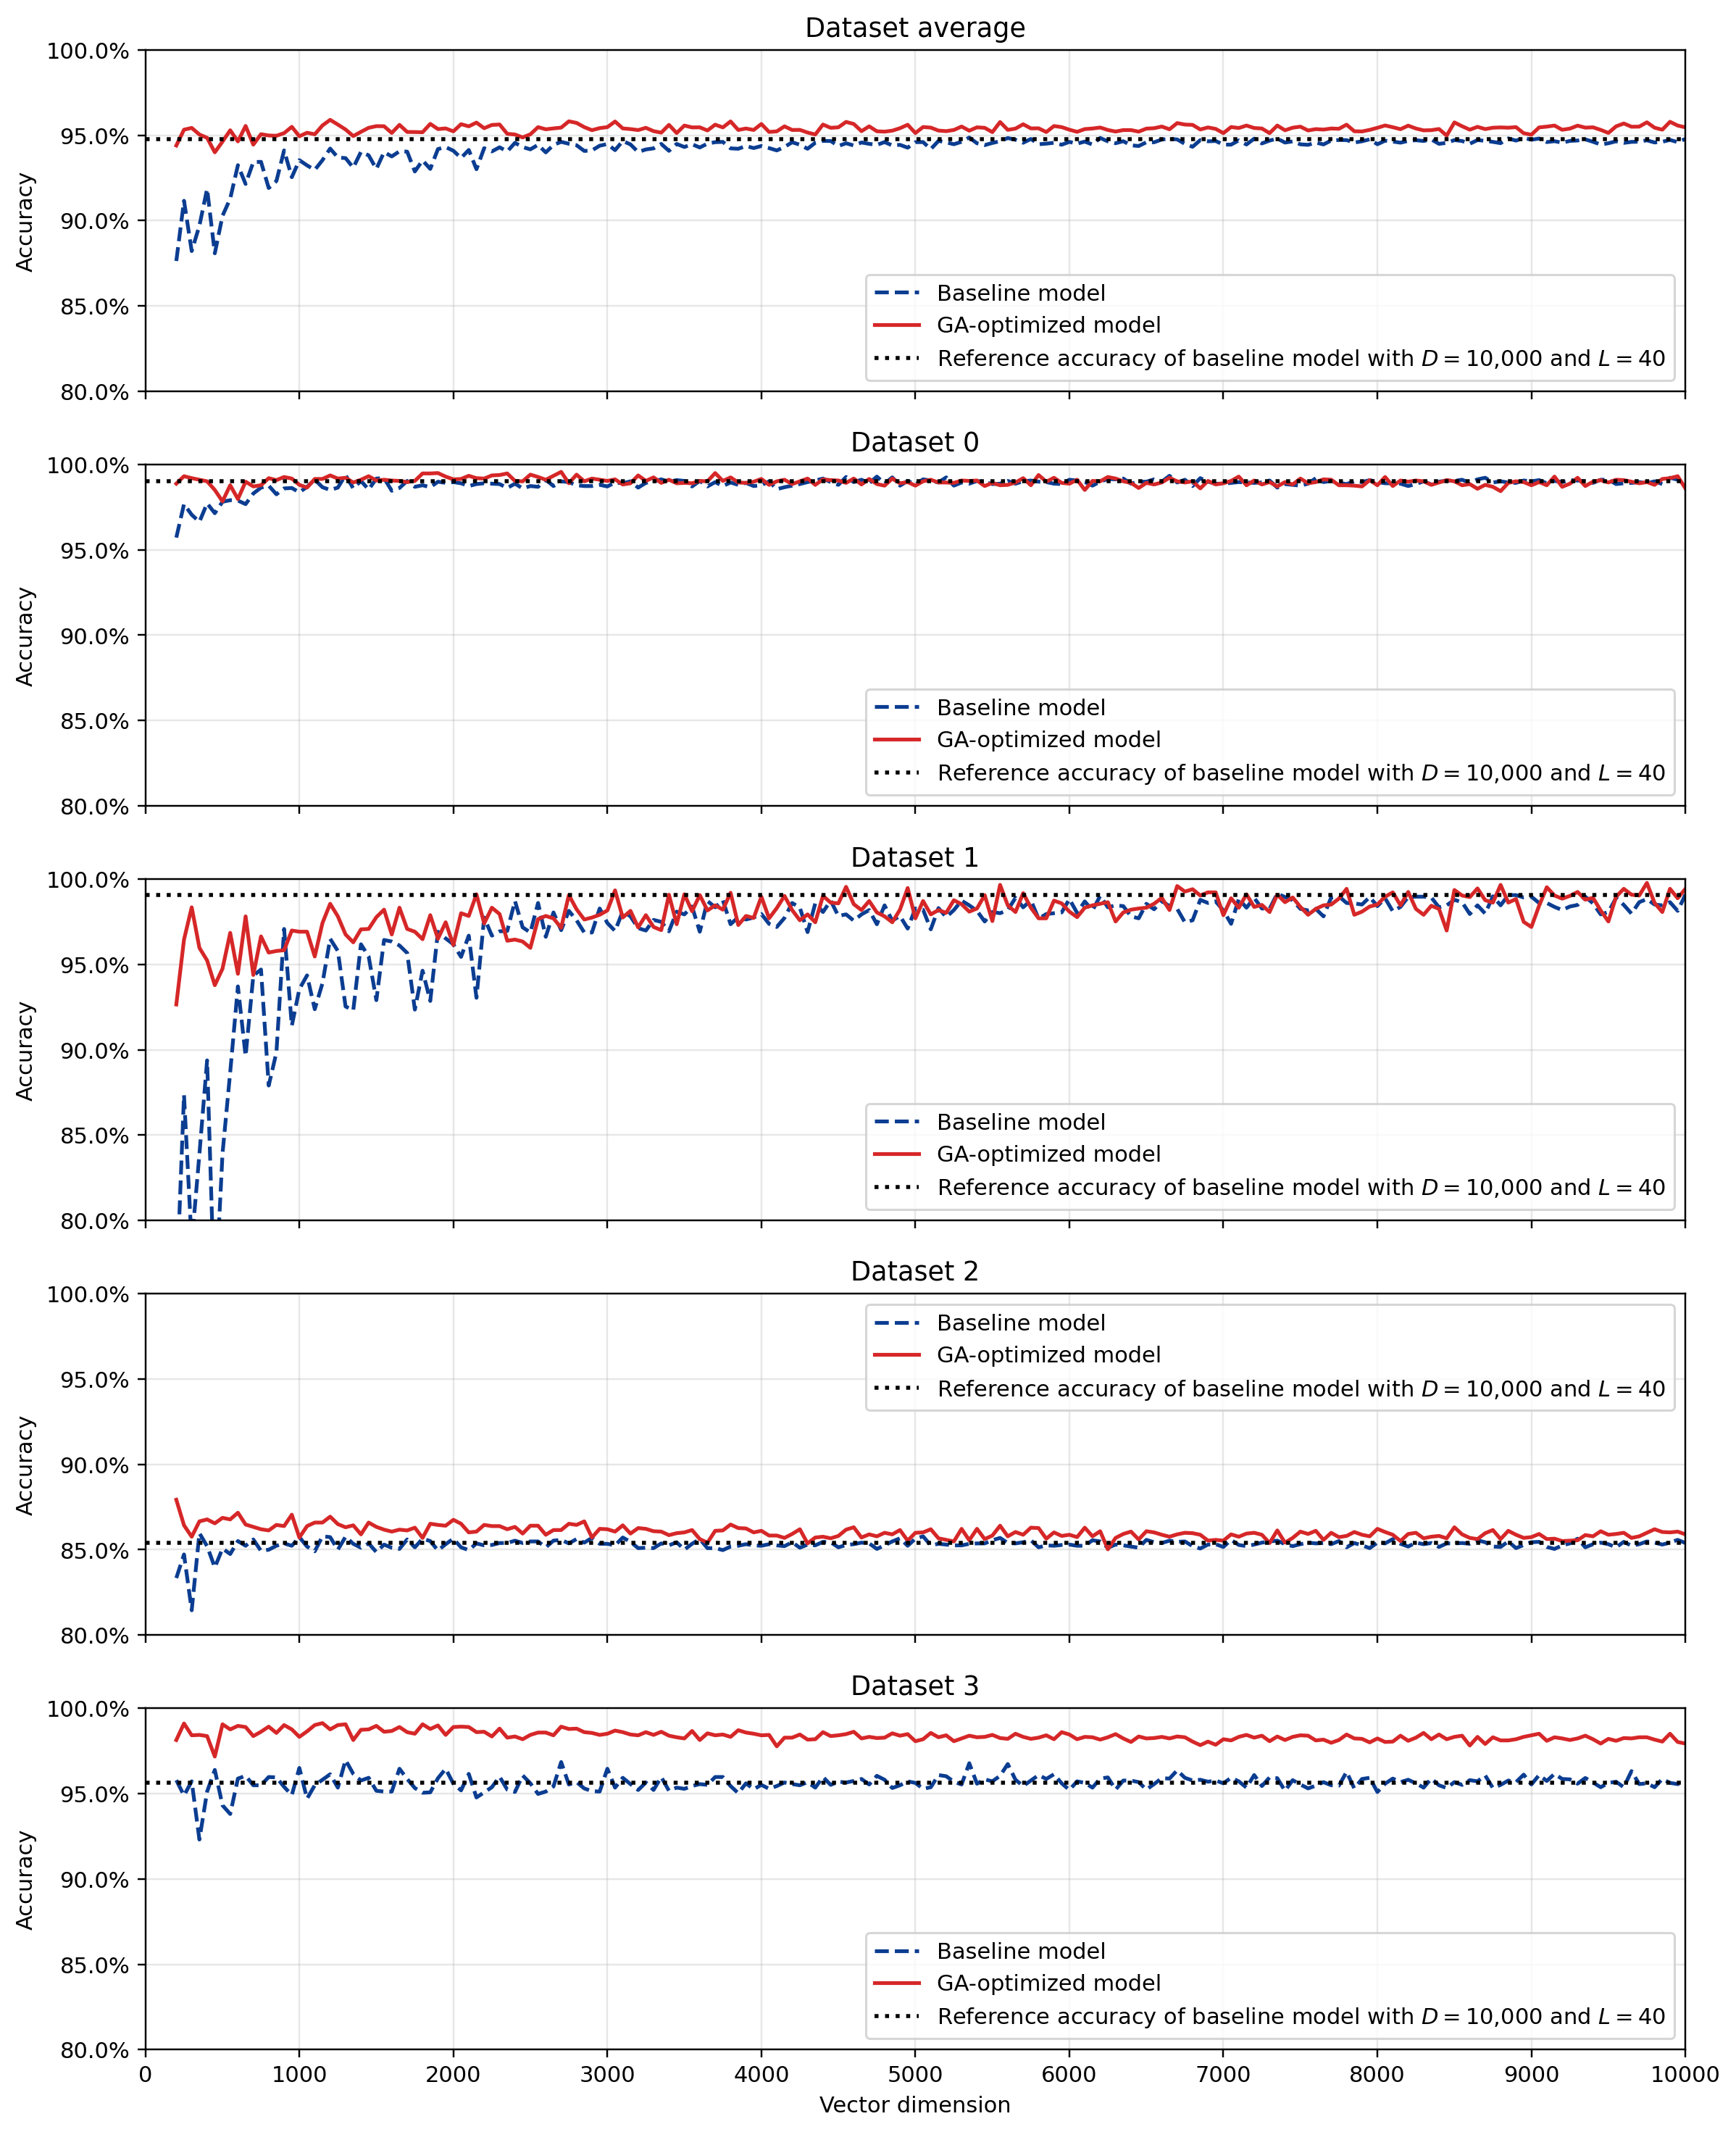
\includegraphics[width=\textwidth]
    {Images/ga_only_comparison.png}
    \caption{Test accuracy of the GA-optimized CCIM (red) compared with the unoptimized equally spaced CCIM (blue) for different vector dimensions at $L=40$. The dotted horizontal line marks the reference accuracy of the unoptimized model with $D=10{,}000$ and $L=40$.}
    \label{fig:ga_only_comparison}
\end{figure} %python3 analysis/benchmarking/GA_only/scripts/plot_pre_vs_post_by_dimension.py --num-levels 40 --min-dimension 0 --max-dimension 10000 --y-min 0.8 --y-max 1.0

\begin{table}[htbp]
    \centering
    \caption{Selected dataset-average test accuracies from the GA-only dimension sweep. The reference is the unoptimized model with $D=10{,}000$ and $L=40$, which achieves $94.78\%$.}
    \label{tab:ga_dimension_summary}
    \begin{tabular}{c c c c c}
        \toprule
        \textbf{$D$}
        & \textbf{Unoptimized}
        & \textbf{GA-optimized}
        & \textbf{Gain}
        & \textbf{GA vs. reference} \\
        \midrule
        201    & 87.63\% & 94.40\% & +6.76 pp & -0.39 pp \\
        251    & 91.16\% & 95.32\% & +4.16 pp & +0.54 pp \\
        501    & 90.28\% & 94.63\% & +4.35 pp & -0.16 pp \\
        701    & 93.43\% & 94.45\% & +1.02 pp & -0.33 pp \\
        751    & 93.44\% & 95.06\% & +1.62 pp & +0.28 pp \\
        1,000  & 93.54\% & 94.94\% & +1.40 pp & +0.16 pp \\
        1,024  & 93.00\% & 95.96\% & +2.96 pp & +1.18 pp \\
        1,050  & 93.23\% & 95.14\% & +1.91 pp & +0.36 pp \\
        10,000 & 94.78\% & 95.46\% & +0.68 pp & +0.68 pp \\
        \bottomrule
    \end{tabular}
\end{table}

The dataset-average result in the top plot of Figure~\ref{fig:ga_only_comparison} and in Table~\ref{tab:ga_dimension_summary} shows that the GA-optimized CCIM improves the test accuracy over the unoptimized CCIM across the evaluated dimension range. The improvement is largest at low dimensions, where the baseline model loses the most accuracy. At $D=201$, the GA increases the dataset-average test accuracy from $87.63\%$ to $94.40\%$, but this still remains slightly below the reference at 94.78\%. Therefore, $D=201$ is still too small if the original reference accuracy should be preserved.

The dataset-average curve exceeds the high-dimensional reference at some low dimensions, but these early crossings are not stable. For example, the optimized model is above the reference at $D=251$, but falls below it again at $D=501$ and $D=701$. Therefore, the first crossing is not used as the selection criterion. Instead, the relevant point is the first dimension after which all larger measured dimensions remain above the reference.
With this criterion, the empirical stability threshold is $D=751$. From this point onward, all larger evaluated dimensions remain above the reference. \\

The dataset-specific plots show that the dataset-average result is not achieved uniformly across all datasets. For Dataset~0, the baseline and reference are already close to saturation at about $99\%$. Consequently, the GA cannot substantially improve the result, but it keeps the reduced-dimensional model close to the reference.

For Dataset~1, the GA improves the low-dimensional configurations substantially, from $75.69\%$ to $92.65\%$ at $D=201$ and from $93.55\%$ to $96.91\%$ at $D=1{,}000$. However, the optimized result at $D=1{,}000$ remains below the Dataset~1 reference accuracy of $99.08\%$. Thus, for this dataset, the GA optimization improves the reduced-dimensional model, but does not fully compensate for the reduction in vector dimension at $L=40$.

Datasets~2 and~3 show a stronger benefit from the GA. For Dataset~2, the GA-optimized model reaches or exceeds its reference for nearly all evaluated dimensions. But the largest improvement relative to the reference is observed for Dataset~3. Already at $D=201$, the optimized model reaches $98.13\%$, compared with the reference of $95.65\%$. Thus, for these datasets, the optimized CCIM not only compensates for reduced vector dimensions, but also improves the accuracy compared with the reference.\\

Overall, the GA-only results show that the optimized CCIM preserves the dataset-average reference accuracy from the empirical stability threshold of $D=751$ onward for all evaluated dimensions. This result does not imply that every dataset individually reaches its own high-dimensional reference, but it shows that the average accuracy can be maintained with a substantially smaller representation. For the FPGA implementation, the reduced dimension is chosen as $D=1{,}024$. Although smaller 64-bit-aligned dimensions above the threshold would also be possible, $D=1{,}024$ is selected because it results in exactly 16 words of 64 bits and provides a convenient power-of-two configuration for the hardware implementation. Compared with the original $D=10{,}000$ configuration, this reduces the hypervector size by a factor of approximately $9.8$, while keeping a margin above the measured stability threshold. Since CCIM storage, associative-memory storage, memory traffic, and the number of vector elements processed by the HDC operations scale directly with $D$, this reduction is highly relevant for the FPGA implementation.




\section{Quantization Results}
\label{sec:quantization_results}

After improving the HDC model with GA optimization and showing that the vector dimension can be reduced while maintaining the dataset-average accuracy, the second optimization approach is evaluated in this section. Instead of optimizing the CCIM hypervectors themselves, this approach changes the quantization boundaries used to map continuous feature values to discrete CCIM levels, as described in Section \ref{sec:quantization}.

As a baseline, uniform binning is used, as in the baseline model and in the previous GA experiments. The method is described in Section~\ref{sec:UniformBinning}. For comparison, the four additional quantization methods described in Sections~\ref{sec:quantileBinning} to~\ref{sec:ChiBinning} are applied. The goal is to adapt the level boundaries so that the resulting levels represent the feature values more meaningfully. If this allows the same accuracy to be reached with fewer levels, the size of the CCIM can be reduced.\\

Before comparing the classification accuracy, the learned quantization boundaries are analyzed directly. Figure~\ref{fig:quantization_threshold_example} shows one example for Dataset~0, feature~15, seed~1, and $L=40$. The upper plot shows for each quantization method at which feature value the level transition boundaries are placed. The lower plot illustrates the value distribution of the feature on which the quantizers are fitted. The grey histogram shows all samples across $L=40$ uniformly spaced bins, while the black curve shows the corresponding \ac{CDF}. In addition, the samples and the \ac{CDF} are shown separately for each class, using one color per class and dashed lines for the class-wise \acp{CDF}.


\begin{figure}[htbp]
    \centering

    % Dataset 0
    \begin{minipage}[t]{0.99\textwidth}
        \centering
        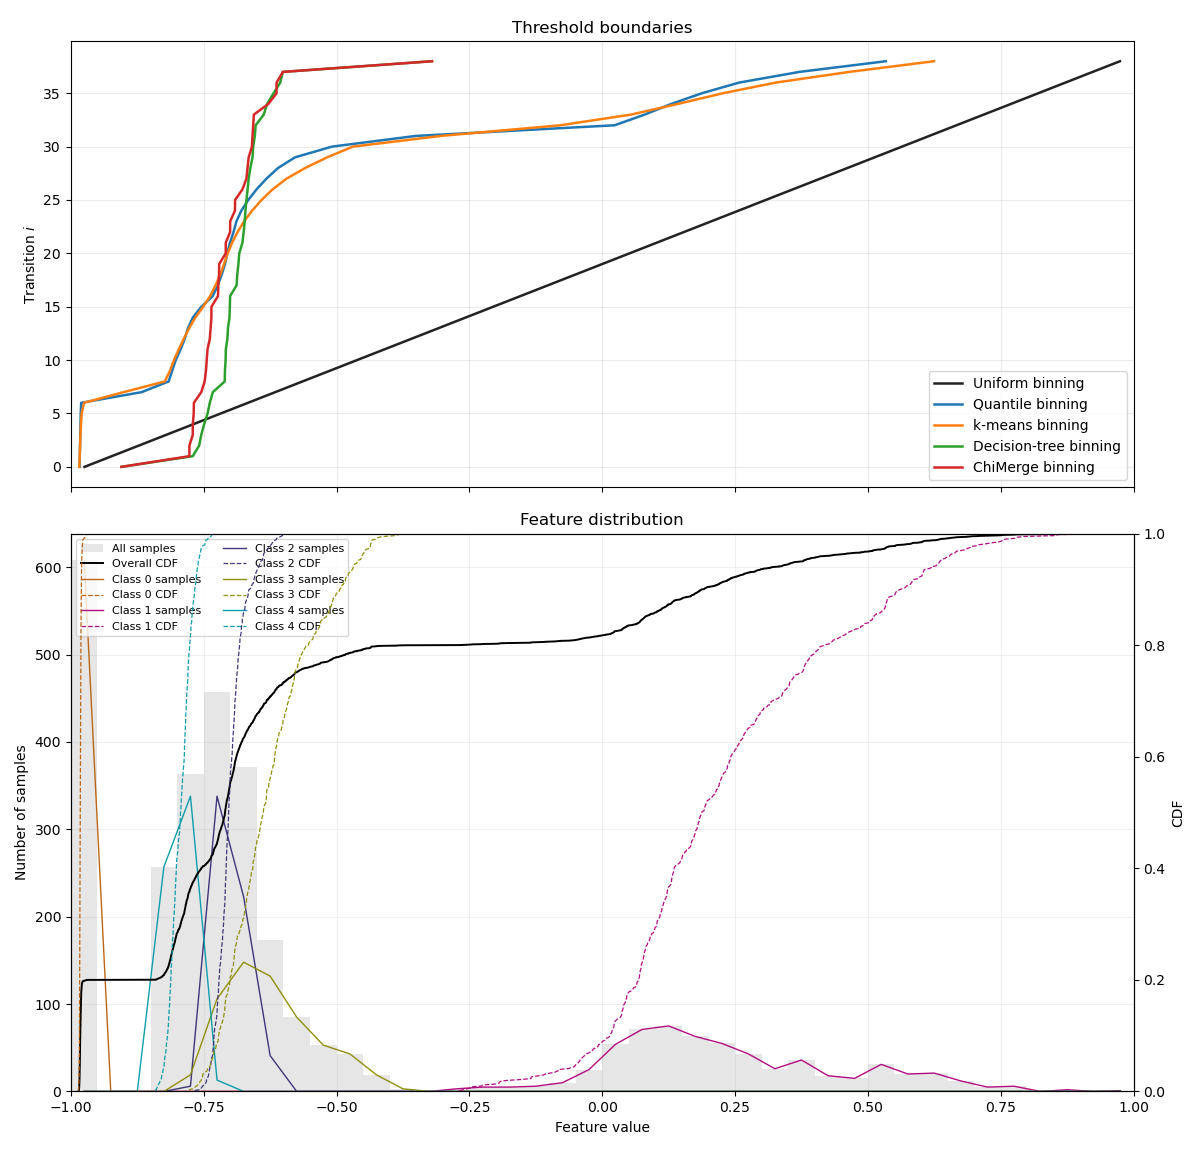
\includegraphics[width=\linewidth]
        {Images/quantizer_histogram.png}
        
    \end{minipage}
    

    \caption{Quantization thresholds and feature-value distribution for Dataset~0, feature~15, seed~1, and $L=40$. The upper plot shows the threshold positions of the different quantization methods. The lower plot shows the corresponding feature distribution, separated by class.}
    \label{fig:quantization_threshold_example}
\end{figure}
%python3 analysis/benchmarking/quantizer_only/threshold_analysis/scripts/plot_thresholds_with_histogram.py \
  %--dataset 0 \
  %--feature 15 \
  %--seed 1 \
  %--num-levels 40 \
  %--vector-dimension 10000 \
  %--methods all

  The feature distribution is strongly non-uniform. Although the histogram range is $[-1,1]$, most samples are concentrated in the negative part of the range. Class~0 forms a very narrow cluster close to $-0.98$, Classes~2, 3, and~4 overlap strongly in the range around $-0.8$ to $-0.6$, and Class~1 is separated from the other classes and extends mainly to values above -0.3 and into the positive range.

This structure explains the different threshold placements of the quantization methods.
Uniform binning distributes the boundaries evenly over the full input range, so the transition thresholds are linearly spaced with respect to the absolute feature value.
Quantile and k-means binning adapt to the sample distribution instead. Since both methods are unsupervised, their threshold distributions are very similar. Both methods concentrate more thresholds in regions with a high sample density, as expected from their dependence on the value distribution. As a result, their thresholds cover a smaller effective value range than uniform quantization. However, the unsupervised methods also assign a considerable part of their thresholds to values above -0.3, which corresponds to the distribution of the samples, but is not necessarily useful for separating the classes in this feature, since this region mainly contains Class~1.

Decision-tree binning and ChiMerge behave differently, because they use the class labels during threshold selection. Both methods place their thresholds only between approximately $-0.90$ and $-0.32$. This means that the class-pure outer regions are not subdivided further, because the samples of Class~0 are mapped below the first threshold, and the samples of Class~1 are mapped above the last threshold. Instead, the available thresholds are concentrated in the region where Classes~2, 3, and~4 overlap and are therefore harder to separate. Thus, the supervised quantizers do not primarily approximate the full feature distribution, but focus their boundaries on class-relevant intervals.

This example shows that adaptive quantization can strongly change the value representation before HDC encoding. However, a more data-adaptive or class-aware threshold distribution does not automatically imply better final accuracy. Therefore, the following experiments evaluate whether these modified boundaries improve the complete HDC classifier.


Figure~\ref{fig:quantizer_level40} compares the different quantization methods for a fixed number of levels $L=40$ and varying vector dimension. The blue dashed curve shows uniform binning as the baseline, while the red, orange, green, and purple curves show quantile binning, k-means binning, decision-tree binning, and ChiMerge binning, respectively. The black dotted line marks the reference accuracy of the uniform baseline model with $D=10{,}000$ and $L=40$. The experiments are evaluated on the test set and averaged over seeds 1 to 5. The plotted dimensions range from $D=201$ to $D=10{,}000$, with a finer spacing of 50 below $D=1{,}000$ and a spacing of 100 dimensions above $D=1{,}000$.


\begin{figure}[htbp]
    \centering
    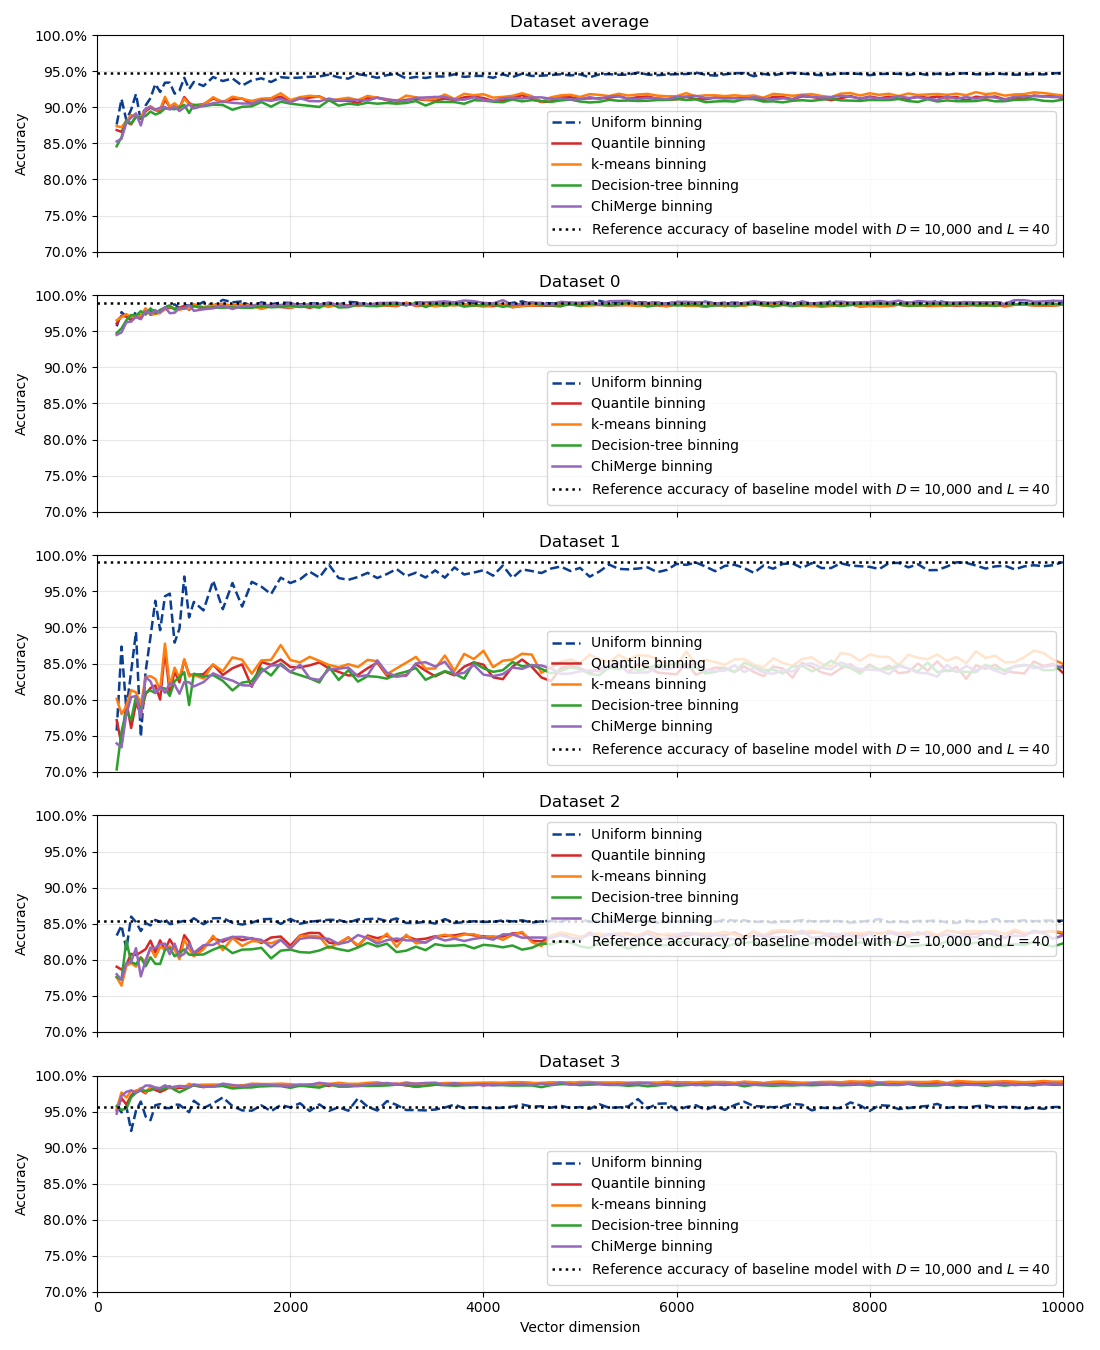
\includegraphics[width=\textwidth]
    {Images/quantizer_only_comparison40.png}
    \caption{Test accuracy of different quantization methods for $L=40$ and varying vector dimension. Uniform binning is shown as the blue dashed baseline. The black dotted line marks the reference accuracy of the uniform baseline model with $D=10{,}000$ and $L=40$.}
    \label{fig:quantizer_level40}
\end{figure}
%python3 analysis/benchmarking/quantizer_only/scripts/plot_pre_vs_baseline_by_dimension.py --num-levels 40 --min-dimension 0 --max-dimension 10000 --y-min 0.7 --y-max 1.0

The results show that the effect of adaptive quantization is highly dataset-dependent. 
For Dataset~0, all methods remain close to the uniform baseline, which indicates that the baseline quantization is already sufficient and leaves little room for improvement.
For Datasets~1 and~2, advanced quantization reduces the accuracy instead of improving it. This effect is strongest for Dataset~1, where even the best adaptive configuration remains far below the uniform reference. Dataset~2 shows a smaller but consistent decrease. Thus, for these datasets, changing the quantization boundaries alone does not produce a more useful HDC representation.
Dataset~3 shows the opposite behavior. Here, all advanced quantizers clearly outperform uniform binning, with k-means binning reaching $99.17\%$ at $D=10{,}000$ compared with the uniform reference of $95.65\%$. This shows that adaptive quantization can substantially improve the HDC classifier for datasets in which the learned boundaries provide a more suitable representation of the feature values.

However, this improvement is not strong enough to compensate for the losses on the other datasets. On the dataset average, all adaptive quantizers remain below the uniform baseline at $L=40$. In addition, none of the adaptive methods reaches the reference accuracy of \(94.78\%\). Therefore, adaptive quantization alone is not sufficient as a replacement for uniform binning.\\

While the previous comparison fixed the number of levels to $L=40$ and varied the vector dimension, Figure~\ref{fig:quantizer_10k} evaluates the opposite direction. Here, the vector dimension is fixed to $D=10{,}000$, while the number of levels is varied from $L=5$ to $L=100$. This experiment tests whether adaptive quantization can reduce the required number of CCIM levels.


\begin{figure}[htbp]
    \centering
    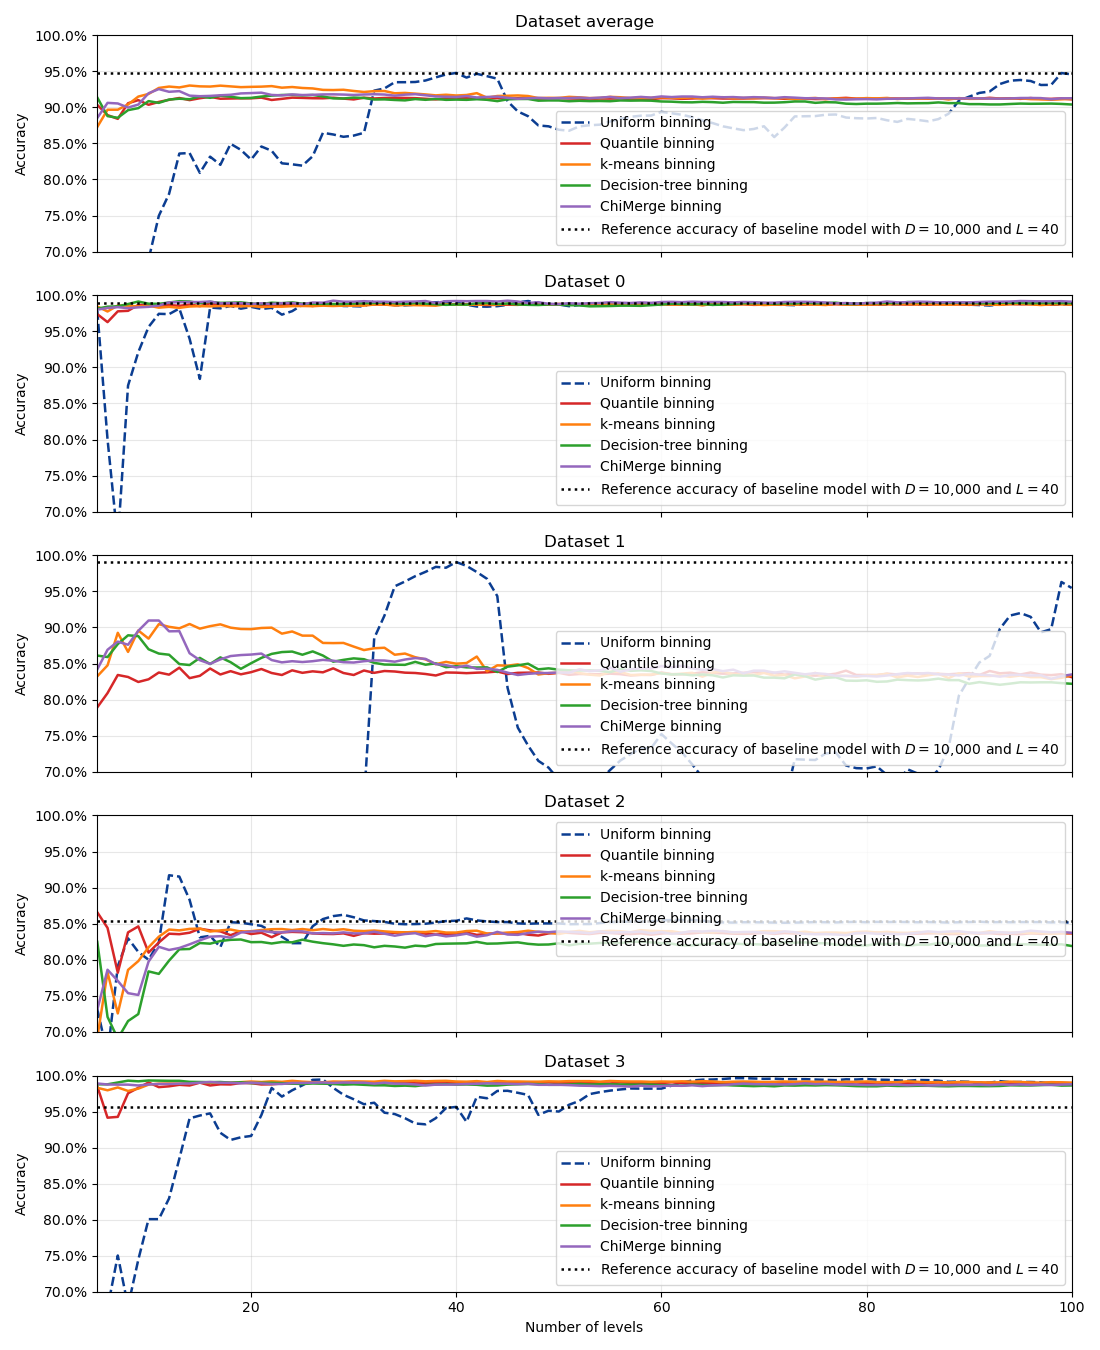
\includegraphics[width=\textwidth]
    {Images/quantizer_only_comparison10k.png}
    \caption{Test accuracy of different quantization methods for $D=10{,}000$ and varying number of levels. Uniform binning is shown as the blue dashed baseline. The black dotted line marks the reference accuracy of the uniform baseline model with $D=10{,}000$ and $L=40$.}
    \label{fig:quantizer_10k}
\end{figure}

The main difference between uniform and adaptive quantization is the dependence on the number of levels. Uniform binning varies strongly with $L$ and shows pronounced peaks and drops, especially for Datasets~1 and~3. In contrast, the adaptive quantizers are much more stable across the tested level range. This indicates that data-dependent thresholds reduce the sensitivity of the HDC model to the exact choice of $L$.

This behavior is especially useful at small numbers of levels. In the dataset average, the adaptive quantizers already reach a similar accuracy at low $L$ as they do at $L=40$, while uniform binning can be much weaker for unfavorable level counts. However, this stability is not sufficient to preserve the fixed reference accuracy. Even the best configuration on the dataset average, k-means binning with $93.04\%$ at $L=14$, remains below the uniform reference of $94.78\%$.

The dataset-specific results confirm the conclusion from the fixed-$L$ comparison in Figure \ref{fig:quantizer_level40}. Dataset~3 benefits clearly from adaptive quantization, and the adaptive methods remain above the reference over almost the entire level range. Dataset~0 is mostly insensitive to the quantization method, except very small level counts. For Datasets~1 and~2, however, adaptive quantization does not provide a reliable improvement over uniform binning. Therefore, the effect of adaptive quantization remains strongly dataset-dependent.

The comparison between the quantization methods shows that no single method is consistently superior. The differences between the methods are smaller than the differences between datasets and smaller than the gap between advanced and uniform quantization at the reference configuration. Averaged over all level counts from $L=5$ to $L=100$ at $D=10{,}000$ and over all datasets, k-means binning performs slightly best with $91.6\%$, while decision-tree binning is lowest with $90.9\%$. Quantile binning and ChiMerge lie between these values. This indicates that the main limitation is not the choice of a specific quantizer, but the fact that adaptive quantization itself is not consistently beneficial across datasets. There is also no clear advantage of supervised over unsupervised methods in this experiment.

Overall, quantization alone reduces the dependence on the exact number of levels, but it does not preserve the reference accuracy on the dataset average. Therefore, it is not sufficient as a standalone method for reducing the number of levels $L$. The result is still useful, because it shows that adaptive thresholds can stabilize configurations with small numbers of levels. The following section therefore evaluates whether this property becomes beneficial when adaptive quantization is combined with GA-based CCIM optimization.

\section{Combined Evaluation and Final Configuration}
\label{sec:combined_results}

The previous sections showed that GA optimization improves the CCIM representation, while adaptive quantization alone does not preserve the reference accuracy on the dataset average. Therefore, this section evaluates whether adaptive quantization becomes useful when combined with GA-based CCIM optimization.

Figure~\ref{fig:combined_comparison} compares the GA-optimized model with uniform binning to GA-optimized models using the four new quantization methods. The number of levels is fixed to $L=40$, while the vector dimension is varied. The dashed blue curve shows the GA-optimized model with uniform binning, the dashed grey curve shows the unoptimized uniform baseline, and the dotted black line marks the reference accuracy of the unoptimized model with $D=10{,}000$ and $L=40$.

\begin{figure}[htbp]
    \centering
    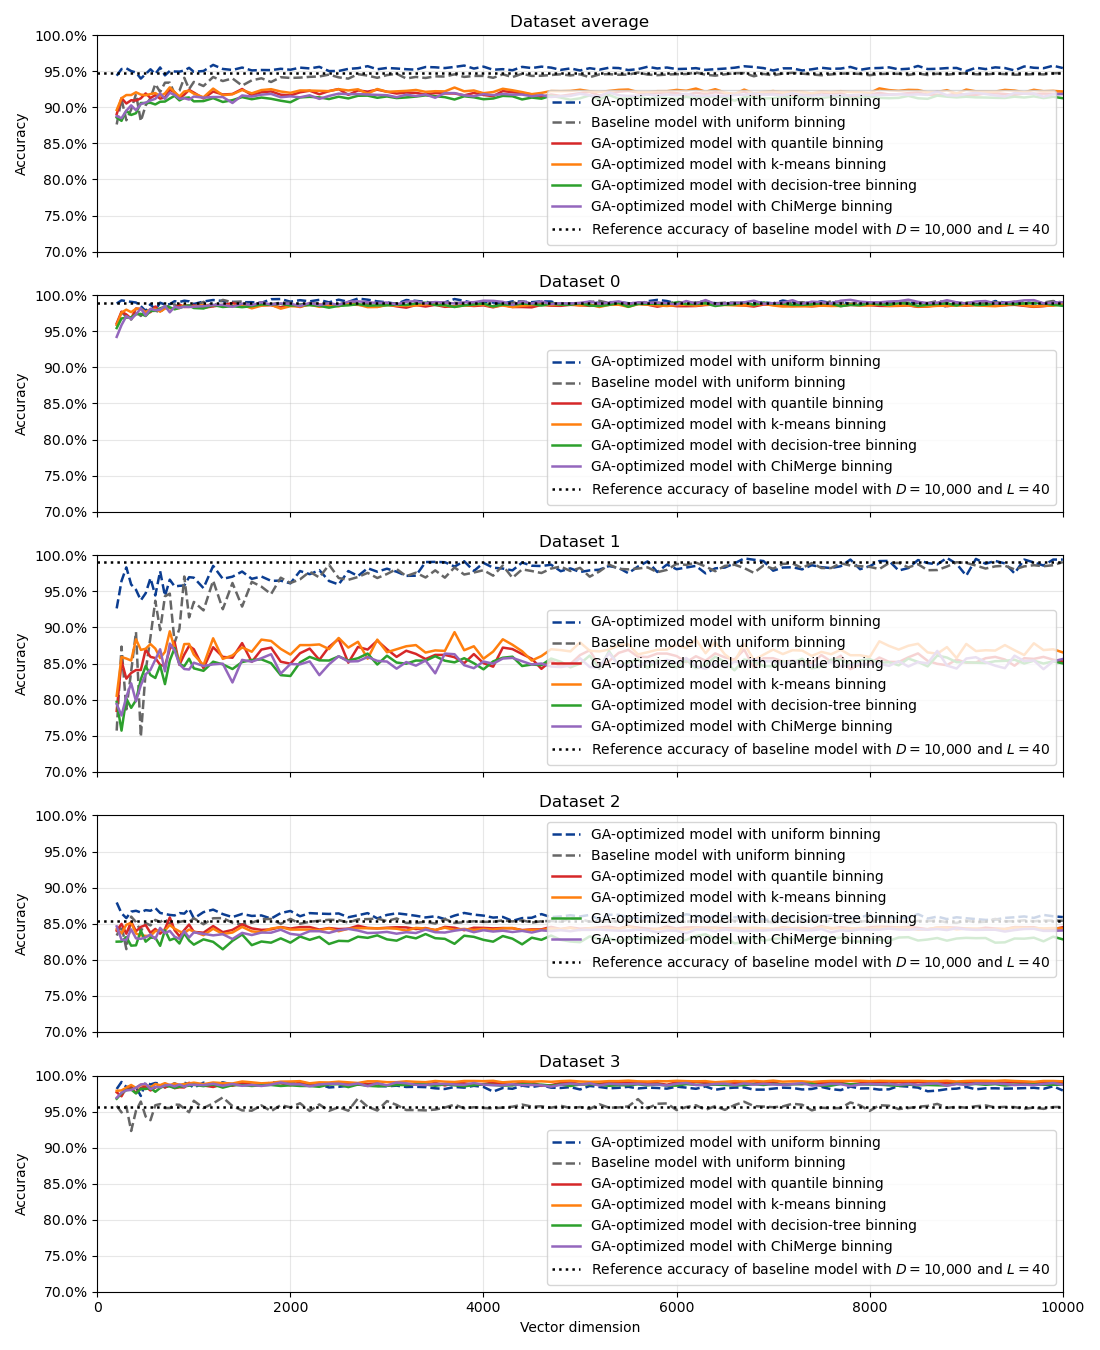
\includegraphics[width=\textwidth]
    {Images/combi_comparison.png}
    \caption{Test accuracy of GA-optimized models with uniform and adaptive quantization for $L=40$ and varying vector dimension. The dashed blue curve shows the GA-optimized model with uniform binning, the dashed grey curve the unoptimized uniform baseline, and the dotted black line the reference accuracy of the unoptimized uniform model with $D=10{,}000$ and $L=40$.}
    \label{fig:combined_comparison}
\end{figure}

The dataset-average result shows that adaptive quantization does not improve the GA-optimized model. The best-performing configuration remains GA optimization with uniform binning, reaching a best measured value of $95.90\%$ in this experiment. In contrast, all GA-optimized adaptive quantizers stay below the reference accuracy of $94.78\%$ on the dataset average. Even the best-performing adaptive combination, k-means binning with GA, reaches a maximum dataset-average accuracy of only $92.79\%$.

The dataset-specific behavior matches the quantization-only results. Dataset~3 benefits from adaptive quantization, but on average across datasets this gain is outweighed by the losses on Datasets~1 and~2. Dataset~0 shows only small differences between the methods. Thus, GA optimization does not remove the dataset dependence of adaptive quantization.

Therefore, adaptive quantization is not used for the final HDC configuration in the FPGA accelerator. Based on the dimension-reduction results in Section \ref{sec:GA_results} and the quantization analysis presented here, the configuration selected for the FPGA evaluation uses uniform binning with $L=40$, a GA-optimized CCIM, and the hardware-aligned vector dimension $D=1{,}024$.


\section{FPGA Accelerator Results}
\label{sec:FPGA_results}

After evaluating the algorithmic optimizations of the HDC model, this section evaluates the FPGA accelerator presented in Section \ref{sec:fpga_accelerator}. The goal is to determine how the optimized model maps to FPGA hardware and which trade-off between processing performance and resource usage results from different degrees of parallelism.

First, the hardware configuration is defined based on the results of the previous sections. Two accelerator variants with different degrees of word-level parallelism are then evaluated. The fully parallelized implementation represents the performance-oriented end of the design space, while the second implementation reduces word-level parallelism to decrease the hardware requirements. Both implementations use the same HDC model and accelerator pipeline, such that the influence of the hardware parallelization can be evaluated independently of the classification model. Finally, the resulting processing performance is compared with the timing requirements of the EMG application.

\subsection{Hardware Configuration}
\label{sec:hardware_config_FPGA}
%Include constants choiced based on previous results. 
% --> derive and describe bit sizes of accelerator data elements. 

The parameters used for the hardware configuration of the accelerator are derived from the results of the previous sections. The GA evaluation identified an empirical stability threshold of $D=751$, above which the dataset-average accuracy remains above the reference when using an optimized \ac{CCIM}. Since the accelerator uses words of width $W=64$ bits and requires the vector dimension to be divisible by the word width, $D=1{,}024$ is selected as a hardware-aligned dimension above the empirical stability threshold.
The number of quantization levels is kept at $L=40$. As shown in Section \ref{sec:quantization_results}, the investigated quantization methods did not preserve the reference accuracy consistently when reducing the number of levels. All other model parameters are kept from the previous sections.

This configuration also determines the widths of the accelerator data types. Representing one of $L=40$ quantization levels requires $w_{\mathrm{level}}=\left\lceil \log_2(40)\right\rceil=6$
bits, while the \(C=5\) classes require $w_{\mathrm{class}}=\left\lceil \log_2(5)\right\rceil=3$ bits. A Hamming distance for $D=1024$ can take values from 0 to 1024 and therefore requires $w_{\mathrm{distance}}=\left\lceil \log_2(D+1) \right\rceil=11$ bits.

Together with the 3-bit command type, the packed accelerator command has a width of
\[
    w_{\mathrm{cmd}}
    =
    3 + w_{\mathrm{class}} + F \cdot w_{\mathrm{level}}
    =
    3 + 3 + 32 \cdot 6
    =
    198~\mathrm{bits}.
\]
For the 32-bit AXI4-Stream interface described in Section~\ref{sec:Axi}, one command therefore requires $\left\lceil \frac{198}{32} \right\rceil=7$ AXI beats. The response consists of one validity bit and one Hamming distance for each class, resulting in

\[
    w_{\mathrm{rsp}}
    =
    1 + C \cdot w_{\mathrm{distance}}
    =
    1 + 5 \cdot 11
    =
    56~\mathrm{bits}.
\]
It is consequently transferred using $\left\lceil \frac{56}{32} \right\rceil=2$ AXI beats. 

The selected vector dimension also reduces the CCIM size compared with the original \(D=10{,}000\) configuration. The CCIM contains \(F \cdot L \cdot D\) bits and therefore requires $32 \cdot 40 \cdot 1024=1{,}310{,}720~\mathrm{bits}=163.84~\mathrm{kB}$, which is smaller by a factor of approximately $9.8$ than in the reference configuration.
The associative memory contains $C=5$ class vectors and therefore requires an additional $5 \cdot 1{,}024 = 5{,}120~\mathrm{bits} = 640~\mathrm{bytes}$.




\subsection{Fully Parallel Implementation}
\label{sec:FullyParallelResults}

To investigate the performance-oriented variant of the accelerator, the fully parallelized implementation is evaluated first.
As described in Section \ref{sec:fpga_accelerator}, the hypervectors are processed in words of 64 bits and the number of words processed in parallel determines the degree of word-level parallelism. In the fully parallelized version, all 16 words are processed in parallel during spatial encoding, class vector accumulation and Hamming distance computation. The target for HLS and FPGA implementation is the XCVU57P-FSVK2892-3-E FPGA with a target clock period of $10~\mathrm{ns}$, corresponding to a clock frequency of $100~\mathrm{MHz}$. The XCVU57P FPGA belongs to AMD's Virtex UltraScale+ HBM family and is designed for high-throughput, data-intensive applications. It provides a generous amount of hardware resources and is therefore well suited for first evaluating the maximum degree of parallelism of the accelerator without strongly restricting the architecture by device capacity \cite{amd_virtex_nodate}.

The generated RTL is verified using the complete sequence of training and inference commands. For all 870 inference samples, the responses, including the validity information and the Hamming distances for all five classes, match the expected outputs. 
The steady-state inference latency, measured from the first AXI command beat until the final AXI response beat, is $52$ clock cycles. At $100~\mathrm{MHz}$, this corresponds to a latency of $0.52~\mathrm{\mu s}$. Due to the pipelined accelerator structure, the processing of consecutive samples overlaps. After the pipeline is filled, inference results are produced at an interval of 12 clock cycles. The resulting steady-state throughput is therefore $\mathrm{TP}_{\mathrm{full}}=\frac{100~\mathrm{MHz}}{12}=8.33~\mathrm{MSamples/s}.$

Detailed stage measurements of the inference path show that the spatial encoding requires six cycles of computation. For valid N-grams, the temporal encoding requires ten cycles and the Hamming distance computation three cycles, while the response generation requires six cycles, followed by two cycles until the second AXI response beat is transferred. In steady-state operation, the spatial encoder can additionally wait up to four cycles for downstream acceptance, resulting in an observed input-to-output latency of up to ten cycles for the spatial encoding stage. Since the pipeline stages operate concurrently, these stage latencies do not add up to the processing interval. Instead, the fully parallelized accelerator produces one inference result every 12 clock cycles.

The implemented design uses $95{,}977$ \acp{LUT}, $48{,}844$ registers and 304 \ac{BRAM} tiles, while no DSP blocks are required. On the XCVU57P FPGA, this corresponds to $7.36~\%$ of the available \acp{LUT}, $1.87~\%$ of the registers and $15.08~\%$ of the \ac{BRAM} resources. The relatively large number of \ac{BRAM} tiles compared with the logical CCIM size is largely caused by the memory banking required for fully parallel access. The logical \ac{CCIM} size remains $163.84~\mathrm{kB}$ as derived in Section \ref{sec:hardware_config_FPGA}, but distributing it across independent memory banks increases the physical memory-resource utilization while enabling all 16 hypervector words to be accessed in parallel. The implementation meets the target clock period of $10~\mathrm{ns}$ with a worst negative slack (WNS) of $+0.803~\mathrm{ns}$ and therefore achieves timing closure at $100~\mathrm{MHz}$.

Although the fully parallelized implementation fits comfortably on the XCVU57P FPGA, this device provides considerably more resources than the smaller FPGA considered for the embedded implementation. Therefore, the accelerator is additionally targeted to the XCZU3EG-SBVA484-1-I FPGA, which belongs to the Zynq UltraScale+ MPSoC family and combines programmable logic with integrated Arm application and real-time processors. It provides $70{,}560$ \acp{LUT}, $141{,}120$ registers and 216 \ac{BRAM} tiles \cite{amd_zynq_2025}. Compared with these resources, the $95{,}977$ \acp{LUT} and 304 \ac{BRAM} tiles required by the fully parallelized implementation on the XCVU57P FPGA already exceed the available LUT and BRAM capacities. Since resource mapping can change when targeting a different FPGA, the design is subsequently synthesized directly for the XCZU3EG. With this target, Vivado reports 608 required RAMB18 primitives compared with 432 available and consequently attempts to map part of the memory to LUT-based storage. This reduces the BRAM requirement to the 216 available tiles, but increases the LUT requirement even further to $116{,}186$, corresponding to $164.66~\%$ of the available LUT capacity. The subsequent placement fails, because the resulting LUT utilization exceeds the device capacity. These results show that the high degree of parallelism imposes excessive requirements on both logic and memory resources for the smaller FPGA. The following implementation therefore reduces the word-level parallelism and adapts the memory banking to the lower number of simultaneously accessed hypervector words.


\subsection{Partially Parallel Implementation}
\label{sec:partParallelResults}

To reduce the resource requirements of the accelerator, the word-level parallelism is reduced in the spatial encoding and class vector accumulation stages. Instead of processing all 16 hypervector words simultaneously, the partially parallelized implementation processes four 64-bit words per cycle. The temporal encoding and Hamming distance computation remain unchanged. Correspondingly, the CCIM memory organization is adapted to the reduced number of simultaneously accessed words, requiring substantially fewer independent memory banks. The implementation is targeted to the XCZU3EG-SBVA484-1-I FPGA introduced in the previous section, while retaining the same target clock frequency of $100~\mathrm{MHz}$.

The generated RTL is again verified using the complete training and inference sequence, with all 870 inference responses matching the expected validity information and Hamming distances. Detailed stage measurements show that the spatial encoding now requires 30 cycles of computation. For valid N-grams, the temporal encoding still requires ten cycles and the Hamming distance computation three cycles, while response generation requires six cycles followed by two cycles for the AXI response transfer. In steady-state operation, one inference result is produced every 32 clock cycles, resulting in a throughput of $\mathrm{TP}_{\mathrm{partial}}=\frac{100~\mathrm{MHz}}{32}=3.125~\mathrm{MSamples/s}.$

For valid inference N-grams, the steady-state latency from the first AXI command beat to the final AXI response beat is 112 clock cycles, corresponding to $1.12~\mathrm{\mu s}$ at $100~\mathrm{MHz}$. The increased latency results primarily from the reduced word-level parallelism of the spatial encoding and the resulting upstream backpressure. As expected, the temporal encoding, distance computation and response generation latencies remain unchanged compared with the fully parallelized implementation.

The implemented design requires $53{,}633$ \acp{LUT}, $38{,}829$ registers and 64 \ac{BRAM} tiles, while again no DSP blocks are used. On the XCZU3EG FPGA, this corresponds to $76.01~\%$ of the available \acp{LUT}, $27.51~\%$ of the registers and $29.63~\%$ of the \ac{BRAM} resources. Despite the considerably smaller device, the implementation therefore fits within the available resources. The target clock period of $10~\mathrm{ns}$ is also met with a WNS of $+0.139~\mathrm{ns}$, confirming timing closure at $100~\mathrm{MHz}$. The reduced parallelism therefore enables implementation on the smaller FPGA, while the resulting resource-performance trade-off is evaluated in detail in the following section.


\subsection{Resource--Performance Trade-off}
\label{sec:FPGAResultsMetrics}

Table \ref{tab:fpga_comparison} summarizes the resource utilization and inference performance of the investigated accelerator implementations. The comparison of the fully and partially parallelized implementations on the XCVU57P FPGA isolates the effect of the reduced word-level parallelism independently of the FPGA model, while the implementation on the XCZU3EG shows the resulting resource usage on the smaller target device.

\begin{table}[ht]
    \centering
    \caption{Resource utilization and inference performance of the fully and partially parallelized accelerator implementations.}
    \label{tab:fpga_comparison}
    \begin{tabular}{lrrr}
        \hline
        Metric & Full, XCVU57P & Partial, XCVU57P & Partial, XCZU3EG \\
        \hline
        LUTs & 95,977 & 49,355 & 53,633 \\
        Registers & 48,844 & 37,685 & 38,829 \\
        BRAM tiles & 304 & 64 & 64 \\
        DSPs & 0 & 0 & 0 \\
        WNS [ns] & +0.803 & +0.667 & +0.139 \\
        Spatial encoding [cycles] & 6 & 30 & 30 \\
        Inference latency [cycles] & 52 & 112 & 112 \\
        Inference interval [cycles] & 12 & 32 & 32 \\
        Throughput [MSamples/s] & 8.33 & 3.125 & 3.125 \\
        \hline
    \end{tabular}
\end{table}

The direct comparison on the XCVU57P shows that reducing the word-level parallelism decreases the LUT requirement from $95{,}977$ to $49{,}355$, corresponding to a reduction of $48.6~\%$, while the number of registers decreases by $22.8~\%$. The strongest reduction is obtained for the memory resources, where the number of BRAM tiles decreases from 304 to 64, or by $78.9~\%$. This reduction results from adapting the CCIM banking to the four simultaneously processed words and is therefore achieved without reducing the logical CCIM size. When implemented on the smaller XCZU3EG, the partially parallelized accelerator requires slightly more LUTs than on the XCVU57P, but remains within the available logic and memory resources and achieves timing closure at $100~\mathrm{MHz}$.

The reduced resource requirements are obtained at the cost of lower inference performance. Processing four instead of 16 hypervector words in parallel increases the spatial encoding computation from 6 to 30 cycles, while the processing times of the other stages remain unchanged. Consequently, the steady-state inference interval increases from 12 to 32 cycles and the throughput decreases from $8.33$ to $3.125~\mathrm{MSamples/s}$. The fully parallelized implementation therefore achieves a $2.67\times$ higher inference throughput, whereas the partially parallelized implementation requires approximately half the LUTs and less than one quarter of the BRAM tiles. The reduced parallelism therefore provides the resource savings required for implementation on the XCZU3EG while retaining the same HDC model and accelerator functionality.


\subsection{Real-Time Suitability}
\label{sec:FPGA_conclusion}

The processing performance of both accelerator variants considerably exceeds the requirements of the EMG application. As described in Section \ref{sec:emg-preprocessing}, the EMG signals are sampled at $2000~\mathrm{Hz}$ and the RMS feature extraction uses a shift of 18 samples between consecutive windows. A new feature vector is therefore generated every $t_{\mathrm{EMG}}=\frac{18}{2000}=9~\mathrm{ms},$ corresponding to an input rate of approximately $111.1$ feature vectors per second. In comparison, the fully parallelized accelerator processes up to $8.33$ million samples per second, while the partially parallelized implementation still achieves $3.125$ million samples per second. The latter therefore provides a throughput margin of approximately $\frac{3.125 \cdot 10^6}{111.1}\approx28{,}125$ relative to the rate at which new feature vectors become available.

The inference latency is similarly small compared with the EMG update interval. At $100~\mathrm{MHz}$, the measured AXI-visible latency of 52 cycles for the fully parallelized implementation corresponds to $0.52~\mathrm{\mu s}$, while the 112 cycles of the partially parallelized implementation correspond to $1.12~\mathrm{\mu s}$. Even after reducing the parallelism sufficiently to fit the XCZU3EG, the accelerator therefore completes the inference of a feature vector several orders of magnitude faster than the $9~\mathrm{ms}$ interval between consecutive feature vectors. The reported values describe the HDC accelerator including its AXI4-Stream interface, but do not include EMG preprocessing, quantization, software control or actuator response. Consequently, the results show that the HDC accelerator itself can process each input within the $9~\mathrm{ms}$ sample interval, while the latency of the complete assistive system remains outside the scope of this evaluation.
